%###############################################################################
%# N1 - Manual - Main                                                          #
%###############################################################################
%#    Copyright 2018 - 2019 Dirk Heisswolf                                     #
%#    This file is part of the N1 project.                                     #
%#                                                                             #
%#    N1 is free software: you can redistribute it and/or modify               #
%#    it under the terms of the GNU General Public License as published by     #
%#    the Free Software Foundation, either version 3 of the License, or        #
%#    (at your option) any later version.                                      #
%#                                                                             #
%#    N1 is distributed in the hope that it will be useful,                    #
%#    but WITHOUT ANY WARRANTY; without even the implied warranty of           #
%#    MERCHANTABILITY or FITNESS FOR A PARTICULAR PURPOSE.  See the            #
%#    GNU General Public License for more details.                             #
%#                                                                             #
%#    You should have received a copy of the GNU General Public License        #
%#    along with N1.  If not, see <http://www.gnu.org/licenses/>.              #
%###############################################################################
%# Version History:                                                            #
%#   November 26, 2018                                                         #
%#      - Initial release                                                      #
%###############################################################################

\documentclass[a4paper,
               titlepage,
               bibliography=totocnumbered]{article}

\usepackage[margin=4cm]{geometry}
\usepackage{float}
\usepackage{fancyhdr}
\usepackage{nameref}
\usepackage{enumitem}
\usepackage{longtable}
\usepackage{multirow}
\usepackage{makecell}
\usepackage{adjustbox}
\usepackage{calc}
\usepackage{graphicx}
\usepackage[table]{xcolor}
\usepackage{pgf}
\usepackage{tikz}
\usepackage{tikz-timing}
\usepackage[colorlinks=true,
            linkcolor=blue,
            citecolor=blue,
            urlcolor=blue,
            bookmarks=true,
            bookmarksopen=true,
            pdftitle={N1 Manual},
            pdfauthor={Dirk Heisswolf},
            pdfdisplaydoctitle=true]{hyperref}
\usepackage[automake, numberedsection, nonumberlist]{glossaries}

%Tables
\makeatletter
\def\nobreakhline{
  \noalign{\ifnum0=`}\fi
    \penalty\@M
    \futurelet\@let@token\LT@@nobreakhline}
\def\LT@@nobreakhline{
  \ifx\@let@token\hline
    \global\let\@gtempa\@gobble
    \gdef\LT@sep{\penalty\@M\vskip\doublerulesep}
  \else
    \global\let\@gtempa\@empty
    \gdef\LT@sep{\penalty\@M\vskip-\arrayrulewidth}
  \fi
  \ifnum0=`{\fi}
  \multispan\LT@cols
     \unskip\leaders\hrule\@height\arrayrulewidth\hfill\cr
  \noalign{\LT@sep}%
  \multispan\LT@cols
     \unskip\leaders\hrule\@height\arrayrulewidth\hfill\cr
  \noalign{\penalty\@M}
  \@gtempa}
\makeatother

\pagestyle{fancy}

%Glossary
\makeglossaries
%###############################################################################
%# N1 - Manual - Glossary                                                      #
%###############################################################################
%#    Copyright 2018 Dirk Heisswolf                                            #
%#    This file is part of the N1 project.                                     #
%#                                                                             #
%#    N1 is free software: you can redistribute it and/or modify               #
%#    it under the terms of the GNU General Public License as published by     #
%#    the Free Software Foundation, either version 3 of the License, or        #
%#    (at your option) any later version.                                      #
%#                                                                             #
%#    N1 is distributed in the hope that it will be useful,                    #
%#    but WITHOUT ANY WARRANTY; without even the implied warranty of           #
%#    MERCHANTABILITY or FITNESS FOR A PARTICULAR PURPOSE.  See the            #
%#    GNU General Public License for more details.                             #
%#                                                                             #
%#    You should have received a copy of the GNU General Public License        #
%#    along with N1.  If not, see <http:%www.gnu.org/licenses/>.               #
%###############################################################################
%# Version History:                                                            #
%#   Novemmber 27, 2018                                                        #
%#      - Initial release                                                      #
%###############################################################################

%Glossary 
\newglossaryentry{ram} {
    name={RAM},
    description={
      Random access memory.
      \nopostdesc
    }
}

\newglossaryentry{forth} {
    name={Forth},
    description={
      Forth is a extensible stack-based programming language.
      \nopostdesc
    }
}
 
\newglossaryentry{byte} {
    name={byte},
    description={
      An 8-bit data entity.
      \nopostdesc
    }
}

\newglossaryentry{word} {
    name={word},
    description={
      The term word  refers to a callable code sequence in \Gls{forth} terminology.
      \nopostdesc
    }
}

\newglossaryentry{jump} {
    name={jump},
    description={
      A change of the program flow without return option.
      \nopostdesc
    }
}

\newglossaryentry{branch} {
    name={conditional branch},
    description={
      A change of the program flow without return option, only if a certain (non-zero)
      argument value is given.
      \nopostdesc
    },
    plural={conditional branches}
}

\newglossaryentry{call} {
    name={call},
    description={
      A change of the program flow, where a return address is kept
      on the \gls{rs}.
      \nopostdesc
    }
}

\newglossaryentry{literal} {
    name={literal},
    description={
      A fixed numerical value within the program code.
      \nopostdesc
    }
}

\newglossaryentry{semicolon} {
    name={;},
    description={
      End of a \gls{word} definition in \Gls{forth}.
      \nopostdesc
    }
}

\newglossaryentry{stack} {
    name={stack},
    description={
      A \gls{lifo} storage.
      \nopostdesc
    }
}

\newglossaryentry{cell} {
    name={cell},
    description={
      A data entity within a \gls{stack}.
      \nopostdesc
    }
}

\newglossaryentry{tos} {
    name={TOS},
    description={
      The top \gls{cell} of a \gls{stack}.
      \nopostdesc
    }
}

\newglossaryentry{rs} {
    name={return stack},
    description={
      A \gls{lifo} storage mainly for maintaining return addresses
      of \glspl{call}.
      \nopostdesc
    }
}

\newglossaryentry{ps} {
    name={parameter stack},
    description={
      A \gls{lifo} storage mainly for keeping call parameters and
      return values.
      \nopostdesc
    }
}

\newglossaryentry{lifo} {
    name={LIFO},
    description={
      A memory which is accessible in last in - first out order.
      \nopostdesc
    }
}

\newglossaryentry{opcode} {
    name={opcode},
    description={
      Encoding of a machine instruction. Short for ``operation code''.
      \nopostdesc
    }
}

\newglossaryentry{alu} {
    name={ALU},
    description={
      Arithmetic Logic Unit.
      \nopostdesc
    }
}

\newglossaryentry{ust} {
    name={UST},
    description={
      A bit field in the stack instruction which contols data movement
      between two neighboring \glspl{cell} in the upper \gls{ps} or \gls{rs}.
      The mnemonic stands for ``\textbf{U}pper \textbf{S}tack \textbf{T}ransition''.
      \nopostdesc
    }
}

\newglossaryentry{ist} {
    name={IST},
    description={
      A bit field in the stack instruction which contols data movement
      on the intermediate \gls{ps} or \gls{rs}.
      The mnemonic stands for
      ``\textbf{I}intermediate \textbf{S}tack \textbf{T}ransition''.
      \nopostdesc
    }
}

\newglossaryentry{ls} {
    name={lower stack},
    description={
      The section of the stack which stored in RAM.
      See \secref{stacks}. 
      \nopostdesc
    }
}

\newglossaryentry{is} {
    name={intermediate stack},
    description={
      The section of the stack, which serves as a buffer between the
      \gls{ls} and the \gls{us}.
      See \secref{stacks}. 
      \nopostdesc
    }
}

\newglossaryentry{us} {
    name={upper stack},
    description={
      The section of the stack, which contains the \gls{tos}. It supports
      reordering of its storage \gls{cell}.
      See \secref{stacks}. 
      \nopostdesc
    }
}

\newglossaryentry{msb} {
    name={MSB},
    description={
      The most significant bit.
      \nopostdesc
    }
}

\newglossaryentry{lsb} {
    name={LSB},
    description={
      The least significant bit.
      \nopostdesc
    }
}

\newglossaryentry{tc} {
    name={throw code},
    description={
      A unique identifier for each type of exception.
      \nopostdesc
    }
}




\begin{document}

%Overline
\makeatletter
\newcommand*{\textoverline}[1]{$\overline{\hbox{#1}}\m@th$}
\makeatother

%Counters
\makeatletter
\renewcommand{\thetable}{\thesection-\@arabic\c@table}
\@addtoreset{table}{section}
\makeatother

\makeatletter
\renewcommand{\thefigure}{\thesection-\@arabic\c@figure}
\@addtoreset{figure}{section}
\makeatother

%References
\newcommand{\secref}[2][Section]{\hyperref[{#2}]{\mbox{#1~\ref*{#2}} \mbox{``\nameref*{#2}``}}}
\newcommand{\tabref}[2][Table]{\hyperref[{#2}]{\mbox{#1~\ref*{#2}}}}
\newcommand{\figref}[2][Figure]{\hyperref[{#2}]{\mbox{#1~\ref*{#2}}}}

%--------------------
% Title
%--------------------
%\title{N1 Manual}
%\date{\today}
%\author{Dirk Heisswolf}
%\maketitle

\begin{titlepage}
  \centering
  
\includegraphics[width=1\textwidth]{./N1_logo.eps} \par
  \vspace{-2cm}
  \LARGE N1 Manual \par
  \vspace{1cm}
  \Large Dirk Heisswolf \par
  \vspace{0.5cm}
  \large \today \par
\end{titlepage}

%--------------------
% Revision history
%--------------------
%###############################################################################
%# N1 - Manual - Revision History                                              #
%###############################################################################
%#    Copyright 2018 Dirk Heisswolf                                            #
%#    This file is part of the N1 project.                                     #
%#                                                                             #
%#    N1 is free software: you can redistribute it and/or modify               #
%#    it under the terms of the GNU General Public License as published by     #
%#    the Free Software Foundation, either version 3 of the License, or        #
%#    (at your option) any later version.                                      #
%#                                                                             #
%#    N1 is distributed in the hope that it will be useful,                    #
%#    but WITHOUT ANY WARRANTY; without even the implied warranty of           #
%#    MERCHANTABILITY or FITNESS FOR A PARTICULAR PURPOSE.  See the            #
%#    GNU General Public License for more details.                             #
%#                                                                             #
%#    You should have received a copy of the GNU General Public License        #
%#    along with N1.  If not, see <http:%www.gnu.org/licenses/>.               #
%###############################################################################
%# Version History:                                                            #
%#   Nowember 26, 2018                                                         #
%#      - Initial release                                                      #
%###############################################################################


\section*{Revision History}
\label{hist}

\begingroup
\setlength{\LTleft}{-20cm plus -1fill}
\setlength{\LTright}{\LTleft}
\begin{center}
  \rowcolors{1}{white}{gray!12}                                         %set alternating row color
  %\begin{longtable}{|r|l|}
  \begin{longtable}{|r|p{80ex}|}
    \rowcolor{white}
    %Header
    \hline                                     
    \rowcolor{gray!25}
    \multicolumn{1}{|c|}{\textbf{\rule{0pt}{2.5ex} Date}}     &  
    \multicolumn{1}{c|}{\textbf{\rule{0pt}{2.5ex}  Change}} \\
    \hline
    \endhead                               
    %Footers
    \hline
    \rowcolor{white}
    \multicolumn{2}{r}{\tiny{...continued}} \\
    \endfoot
    \hline
    \endlastfoot
    %Revisions
     March 21, 2019 & Initial release \\   
     March 22, 2019 & Changed encoding of ALU operands 
     (see \tabref{opcodes:alu:operators} and \tabref{words:list})  \\   
     April 17, 2019 & Fixed some copy \& paste errors \\ 
     April 26, 2019 & Fixes and a description of the branch condition in \secref{opcodes:branch} \\ 
%    \today & Pre-release \\   
  \end{longtable}
\end{center}  
\endgroup


%--------------------
% Table of Contents
%--------------------
\setcounter{tocdepth}{2}
\tableofcontents
\pagebreak
\listoffigures
\pagebreak
\listoftables

%--------------------
% Overview
%--------------------
%###############################################################################
%# N1 - Manual - Overview                                                      #
%###############################################################################
%#    Copyright 2018 Dirk Heisswolf                                            #
%#    This file is part of the N1 project.                                     #
%#                                                                             #
%#    N1 is free software: you can redistribute it and/or modify               #
%#    it under the terms of the GNU General Public License as published by     #
%#    the Free Software Foundation, either version 3 of the License, or        #
%#    (at your option) any later version.                                      #
%#                                                                             #
%#    N1 is distributed in the hope that it will be useful,                    #
%#    but WITHOUT ANY WARRANTY; without even the implied warranty of           #
%#    MERCHANTABILITY or FITNESS FOR A PARTICULAR PURPOSE.  See the            #
%#    GNU General Public License for more details.                             #
%#                                                                             #
%#    You should have received a copy of the GNU General Public License        #
%#    along with N1.  If not, see <http://www.gnu.org/licenses/>.              #
%###############################################################################
%# Version History:                                                            #
%#   Novemmber 26, 2018                                                        #
%#      - Initial release                                                      #
%###############################################################################

\section{Overview}
\label{overview}

The N1 is a 16-bit stack machine, targeted for low-end FPGA applications.
Its instruction set and architecture are designed for efficient execution
of \Gls{forth} code. 

\noindent
Here is a summary of the N1's characteristics:

\begin{description}[style=nextline]

%Memory connection  
\item[Memory connection:]  
  \begin{itemize}
  \item[]
  \item 16-bit \gls{vna}
  \item Separate address space for \gls{stack} content
  \item \Gls{wb} interfaces to main and stack memory 
  \item Up to 128KB (main) memory space
  \item Memory addressable in 16-bit entities only
  \end{itemize}

%Stacks  
\item[Stacks:]
  \begin{itemize}
  \item[]
  \item Two hardware \glspl{stack} (\glslink{ps}{parameter} and \gls{rs})
  \item Each \gls{stack} consists of three segments:
    \begin{description}[style=nextline]
    %Upper stack  
    \item[\Gls{us}:]
      \begin{itemize}
      \item[]
      \item Shift registers with selectable shift direction for each individual cell
      \item Fixed size
        \begin{itemize}
        \item Upper \gls{ps}: 4 \glspl{cell}
        \item Upper \gls{rs}: 1 \gls{cell}
        \end{itemize}
      \end{itemize}
    %Intermediate stack  
    \item[\Gls{is}:]
      \begin{itemize}
      \item[]
      \item Buffer with lazy data transfers to and from the lower stack
      \item Configurable size
      \end{itemize}
    %Lower stack
    \item[\Gls{ls}:]
      \begin{itemize}
      \item[]
      \item \gls{ram} space shared by both \glspl{stack}
      \item \Glspl{stack} grow towards each other
      \item Up to 128KB in size
      \end{itemize}
    \end{description}
  \end{itemize}

%Instruction set  
\item[Instruction set:]
  \begin{itemize}
  \item[]
  \item Fixed instruction size of 16-bit
  \item \Glspl{jump} and \glspl{call}
    \begin{itemize}
    \item \Gls{indadr}
    \item \Gls{diradr} within a 32KB window
    \item Two bus cycle execution time
    \item Return from \glspl{call} performed concurrently with last instruction
    \end{itemize}
  \item \Glspl{branch}
    \begin{itemize}
    \item \glslink{diradr}{Direct} \gls{reladr} within a 16KB range
    \item Two bus cycles of execution time if branch is taken, one cycle if not
    \end{itemize}         
  \item \Glspl{literal}
    \begin{itemize}
    \item \glslink{immop}{Immediate} encoding of literals between -2048 and 2047
    \item Literals out of this range requre one additional instruction
    \end{itemize}
  \item \glslink{alu}{Arithmetic and logic operations}
    \begin{itemize}
    \item Single cycle \Gls{alu} operations include:
      \begin{itemize}
      \item Sum and Difference
      \item Comparisons
      \item Signed and unsigned products
      \item Bitwise logic operations
      \item Milti-bit shifts
     \end{itemize}
    \item Optional \glslink{immop}{immediate} encoding of one operand, using
      5-bit encoding 
    \end{itemize}
  \item \Gls{stack} operations
    \begin{itemize}
      \item All 1024 stack transitions of the \gls{us} encodable
    \end{itemize}
  \item Memory I/O
    \begin{itemize}
    \item \Gls{indadr}
    \item \Gls{diradr} within a 511B window
    \item Two bus cycle execution time if branch is taken, one cycle if not
    \end{itemize}   
  \end{itemize}

%Exceptions
\item[Exceptions:]
  \begin{itemize}
  \item[]
  \item Exception handler invoked by five error conditions:
    \begin{itemize}
    \item \Gls{ps} overflow
    \item \Gls{ps} underflow
    \item \Gls{rs} overflow
    \item \Gls{rs} underflow
    \item Access violations in the (main) address space
    \end{itemize}
  \end{itemize}
    
%Interrupts  
\item[Interrupts:]
  \begin{itemize}
  \item[]
  \item Optional interrupt support through external interrupt controller
  \item Automatic interrupt acknowledge (flag clearing) supported
  \end{itemize}
  
\end{description}


%--------------------
% Instruction set
%--------------------
%###############################################################################
%# N1 - Manual - Instruction set                                               #
%###############################################################################
%#    Copyright 2018 Dirk Heisswolf                                            #
%#    This file is part of the N1 project.                                     #
%#                                                                             #
%#    N1 is free software: you can redistribute it and/or modify               #
%#    it under the terms of the GNU General Public License as published by     #
%#    the Free Software Foundation, either version 3 of the License, or        #
%#    (at your option) any later version.                                      #
%#                                                                             #
%#    N1 is distributed in the hope that it will be useful,                    #
%#    but WITHOUT ANY WARRANTY; without even the implied warranty of           #
%#    MERCHANTABILITY or FITNESS FOR A PARTICULAR PURPOSE.  See the            #
%#    GNU General Public License for more details.                             #
%#                                                                             #
%#    You should have received a copy of the GNU General Public License        #
%#    along with N1.  If not, see <http://www.gnu.org/licenses/>.              #
%###############################################################################
%# Version History:                                                            #
%#   November 26, 2018                                                         #
%#      - Initial release                                                      #
%###############################################################################

\section{Instruction Set}
\label{opcodes}

All N1 CPU uses the following instruction encoding:

\begin{figure}[!h]
  %\begin{center}
  \makebox[\textwidth][c]{
    \scalebox{0.8} {
      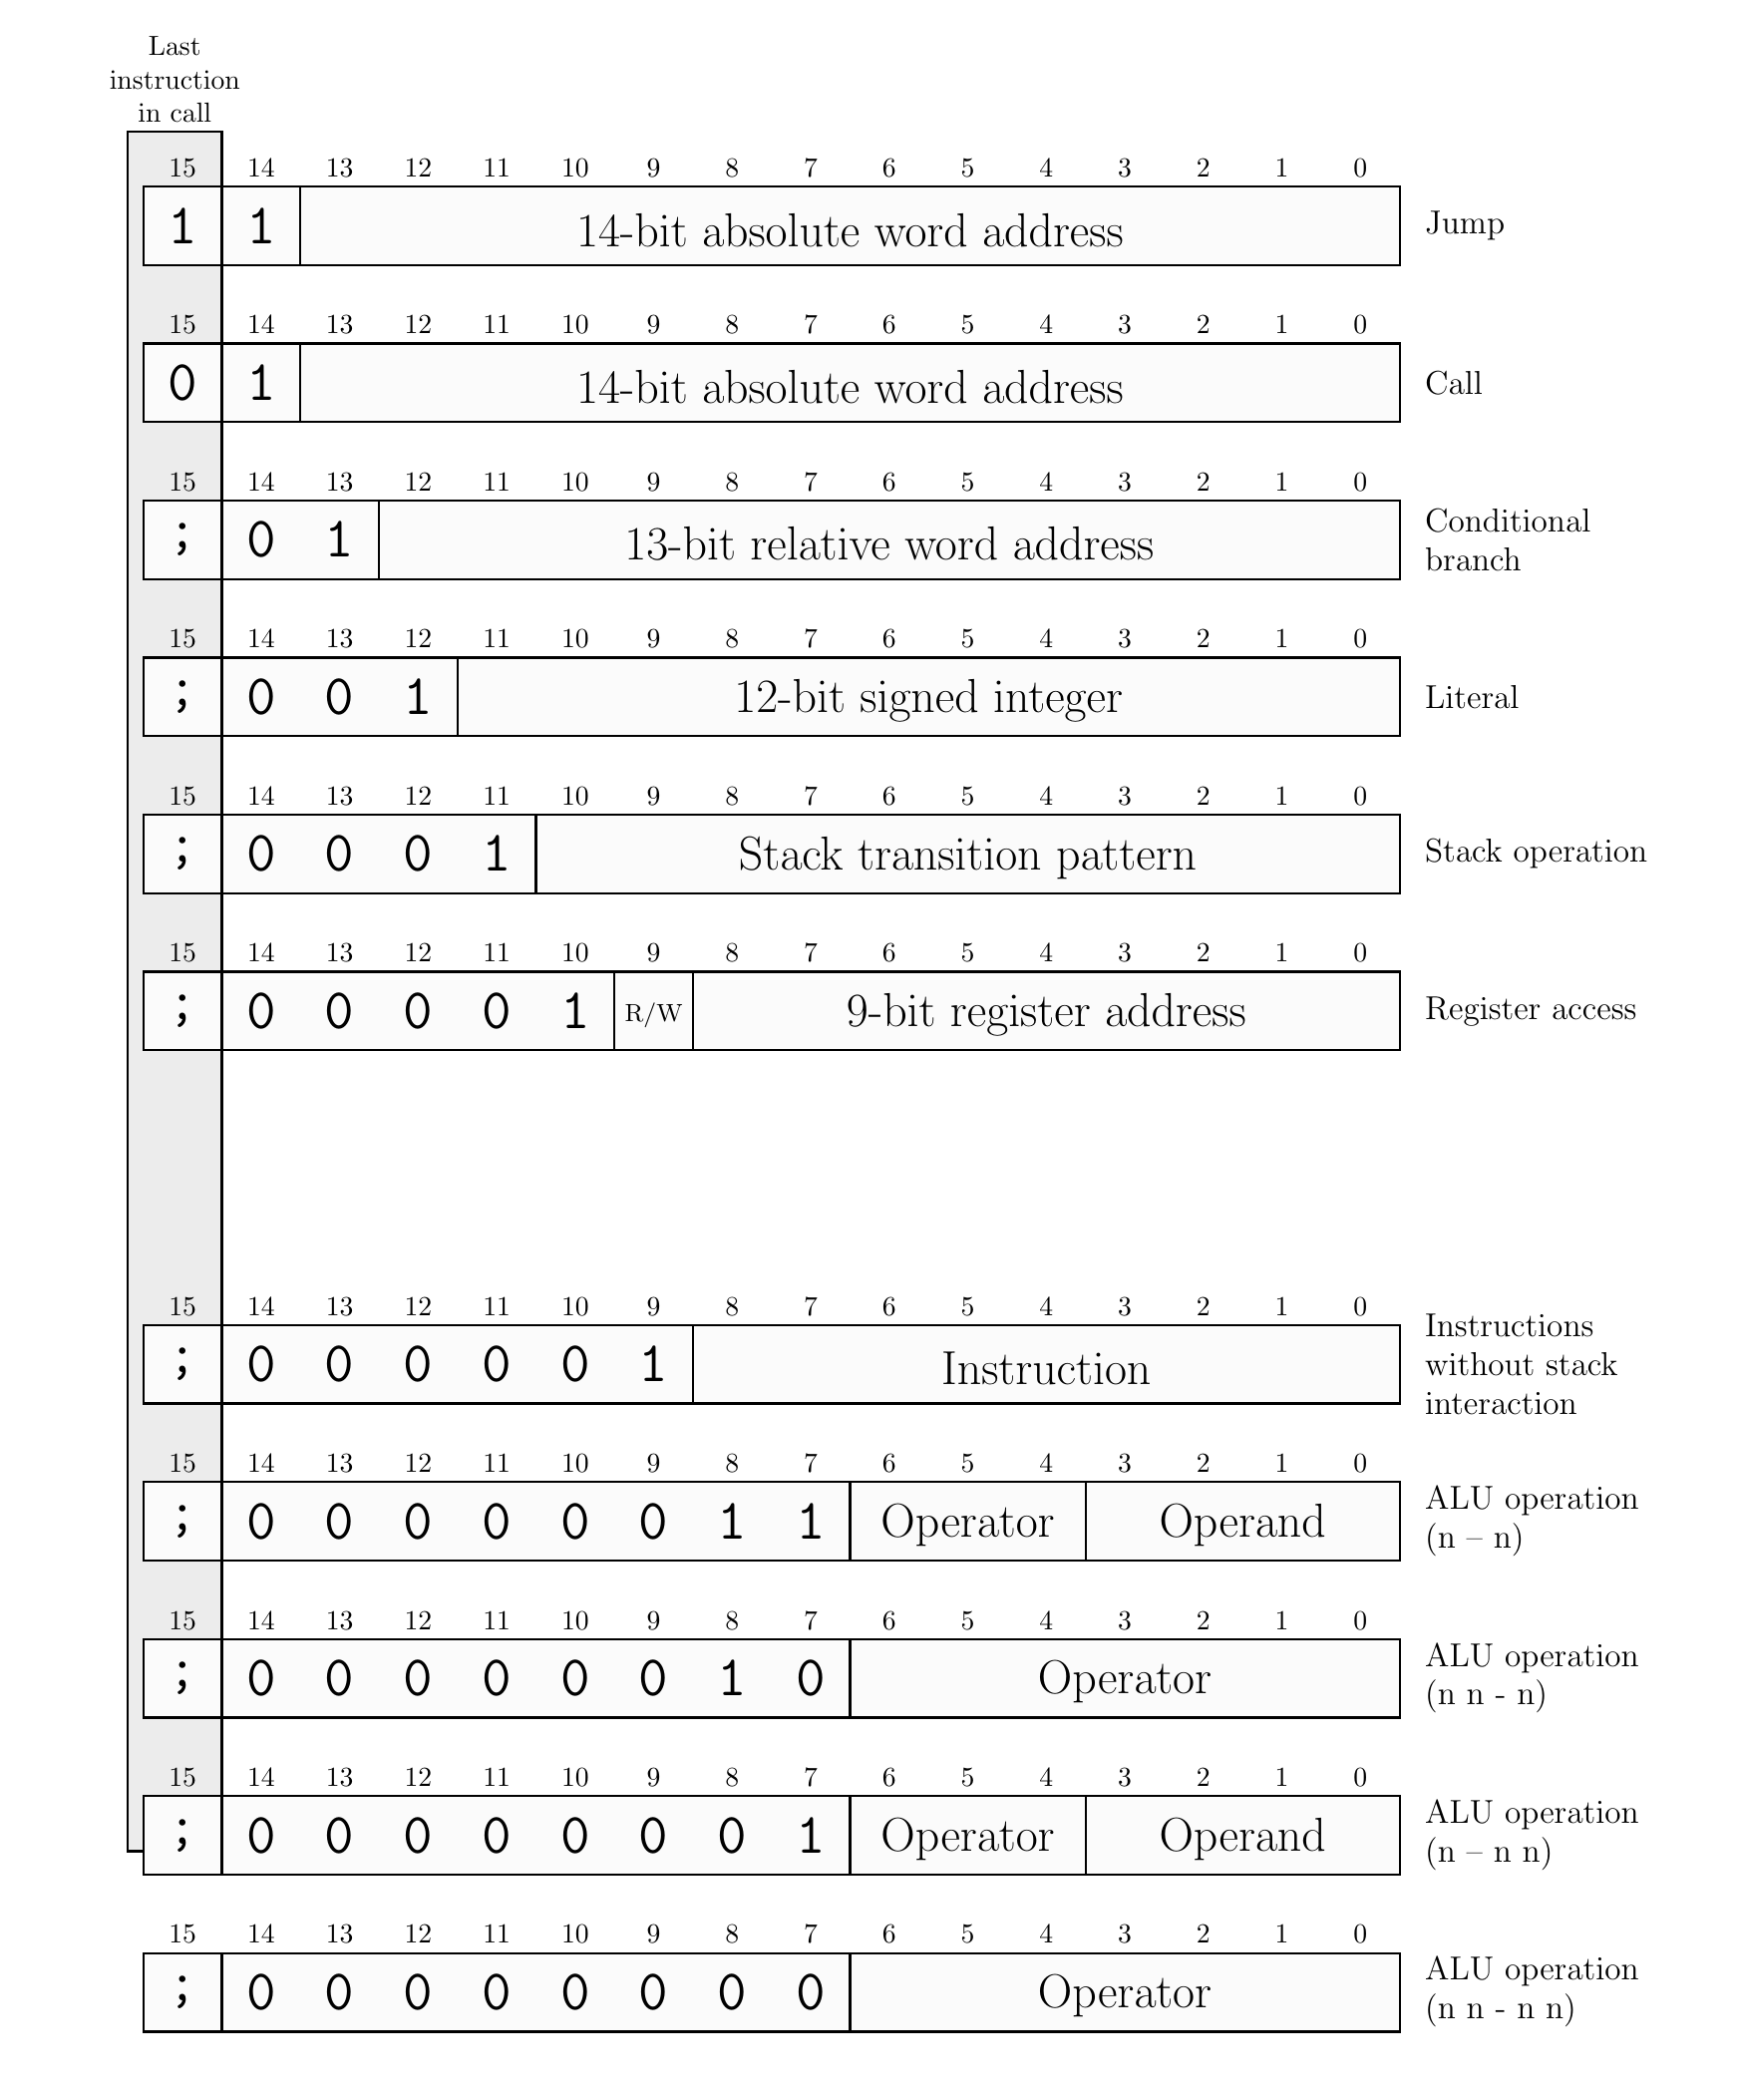
\begin{tikzpicture}
      
        %Instruction
        \newsavebox{\instruction}
        \savebox{\instruction}{
          \draw [thick, fill=gray!3] (0,0) rectangle (16,1);
          \draw [thick, fill=gray!3] (0,0) rectangle (1,1);
          \node [above] at (0.5,1)  {15};
          \node [above] at (1.5,1)  {14};
          \node [above] at (2.5,1)  {13};
          \node [above] at (3.5,1)  {12};
          \node [above] at (4.5,1)  {11};
          \node [above] at (5.5,1)  {10};
          \node [above] at (6.5,1)  {9};
          \node [above] at (7.5,1)  {8};
          \node [above] at (8.5,1)  {7};
          \node [above] at (9.5,1)  {6};
          \node [above] at (10.5,1) {5};
          \node [above] at (11.5,1) {4};
          \node [above] at (12.5,1) {3};
          \node [above] at (13.5,1) {2};
          \node [above] at (14.5,1) {1};
          \node [above] at (15.5,1) {0};
        };

        %Return bit
        \draw [thick, fill=gray!15] (0.8,2.8) rectangle (2,24.7);
        \node [above] at (1.4,24.7) {
          \begin{minipage}[c]{10em}
            \begin{center}
              Last \\
              instruction \\
              in call
            \end{center}
          \end{minipage}};
      
        %Jump
        \node at (1,23) {\usebox{\instruction}};
        \node         at (1.5,23.5)   {\huge{\texttt{1}}};
        \draw [thick] (2,23) rectangle (3,24);
        \node         at (2.5,23.5)   {\huge{\texttt{1}}};
        \node         at (10,23.45)   {\LARGE{14-bit absolute word address}};
        \node [right] at (17.2,23.5)  {\large{Jump}};
     
        %Call
        \node at (1,21) {\usebox{\instruction}};
        \node         at (1.5,21.5)   {\huge{\texttt{0}}};
        \draw [thick] (2,21) rectangle (3,22);
        \node         at (2.5,21.5)   {\huge{\texttt{1}}};
        \node         at (10,21.45)   {\LARGE{14-bit absolute word address}};
        \node [right] at (17.2,21.5)  {\large{Call}};
       
        %Conditional Branch
        \node at (1,19) {\usebox{\instruction}};
        \node         at (1.5,19.5)   {\huge{\texttt{;}}};
        \draw [thick] (2,19) rectangle (4,20); 
        \node         at (2.5,19.5)   {\huge{\texttt{0}}};
        \node         at (3.5,19.5)   {\huge{\texttt{1}}};
        \node         at (10.5,19.45) {\LARGE{13-bit relative word address}};
        \node [right] at (17.2,19.5)  {
          \begin{minipage}[l]{10em}
            \large{
              Conditional \\
              branch
            }
        \end{minipage}};
        
        %Literal 
        \node at (1,17) {\usebox{\instruction}};
        \node         at (1.5,17.5)   {\huge{\texttt{;}}};
        \draw [thick] (2,17) rectangle (5,18); 
        \node         at (2.5,17.5)   {\huge{\texttt{0}}};
        \node         at (3.5,17.5)   {\huge{\texttt{0}}};
        \node         at (4.5,17.5)   {\huge{\texttt{1}}};
        \node         at (11,17.45)   {\LARGE{12-bit signed integer}};
        \node [right] at (17.2,17.5)  {\large{Literal}};

        %Stack operation 
        \node at (1,15) {\usebox{\instruction}};
        \node         at (1.5,15.5)   {\huge{\texttt{;}}};
        \draw [thick] (2,15) rectangle (6,16); 
        \node         at (2.5,15.5)   {\huge{\texttt{0}}};
        \node         at (3.5,15.5)   {\huge{\texttt{0}}};
        \node         at (4.5,15.5)   {\huge{\texttt{0}}};
        \node         at (5.5,15.5)   {\huge{\texttt{1}}};   
        \node         at (11.5,15.45) {\LARGE{Stack transition pattern}};
        \node [right] at (17.2,15.5)  {\large{Stack operation}};
        
        %Register access
        \node at (1,13) {\usebox{\instruction}};
        \node         at (1.5,13.5)   {\huge{\texttt{;}}};
        \draw [thick] (2,13) rectangle (7,14); 
        \draw [thick] (7,13) rectangle (8,14); 
        \node         at (2.5,13.5)   {\huge{\texttt{0}}};
        \node         at (3.5,13.5)   {\huge{\texttt{0}}};
        \node         at (4.5,13.5)   {\huge{\texttt{0}}};
        \node         at (5.5,13.5)   {\huge{\texttt{0}}};   
        \node         at (6.5,13.5)   {\huge{\texttt{1}}};   
        \node         at (7.5,13.45)  {\small{R/\textoverline{W}}};   
        \node         at (12.5,13.45) {\LARGE{9-bit register address}};
        \node [right] at (17.2,13.5)  {\large{Register access}};

        %Control Instructions
        \node at (1,8.5) {\usebox{\instruction}};
        \node         at (1.5,9)       {\huge{\texttt{;}}};
        \draw [thick] (2,8.5) rectangle (8,9.5); 
        \node         at (2.5,9)       {\huge{\texttt{0}}};
        \node         at (3.5,9)       {\huge{\texttt{0}}};
        \node         at (4.5,9)       {\huge{\texttt{0}}};
        \node         at (5.5,9)       {\huge{\texttt{0}}};   
        \node         at (6.5,9)       {\huge{\texttt{0}}};   
        \node         at (7.5,9)       {\huge{\texttt{1}}};   
        \node         at (12.5,8.95)  {\LARGE{Instruction}};
        \node [right] at (17.2,9) {
          \begin{minipage}[l]{10em}
            \large{
              Instructions \\
              without stack \\
              interaction
            }
        \end{minipage}};
            
        %ALU operation (n -- n) 
        \node at (1,6.5) {\usebox{\instruction}};
        \node         at (1.5,7)      {\huge{\texttt{;}}};
        \draw [thick] (2,6.5) rectangle (10,7.5); 
        \draw [thick] (10,6.5) rectangle (13,7.5); 
        \node         at (2.5,7)      {\huge{\texttt{0}}};
        \node         at (3.5,7)      {\huge{\texttt{0}}};
        \node         at (4.5,7)      {\huge{\texttt{0}}};
        \node         at (5.5,7)      {\huge{\texttt{0}}};   
        \node         at (6.5,7)      {\huge{\texttt{0}}};   
        \node         at (7.5,7)      {\huge{\texttt{0}}};   
        \node         at (8.5,7)      {\huge{\texttt{1}}};   
        \node         at (9.5,7)      {\huge{\texttt{1}}};   
        \node         at (11.5,6.95)  {\LARGE{Operator}};
        \node         at (15,6.95)    {\LARGE{Operand}};
        \node [right] at (17.2,7) {
          \begin{minipage}[l]{10em}
            \large{
              ALU operation \\
              (n -- n)
            }
        \end{minipage}};
               
        %ALU operation (n n -- n) 
        \node at (1,4.5) {\usebox{\instruction}};
        \node         at (1.5,5)      {\huge{\texttt{;}}};
        \draw [thick] (2,4.5) rectangle (10,5.5); 
        \node         at (2.5,5)      {\huge{\texttt{0}}};
        \node         at (3.5,5)      {\huge{\texttt{0}}};
        \node         at (4.5,5)      {\huge{\texttt{0}}};
        \node         at (5.5,5)      {\huge{\texttt{0}}};   
        \node         at (6.5,5)      {\huge{\texttt{0}}};   
        \node         at (7.5,5)      {\huge{\texttt{0}}};   
        \node         at (8.5,5)      {\huge{\texttt{1}}};   
        \node         at (9.5,5)      {\huge{\texttt{0}}};   
        \node         at (13.5,4.95)  {\LARGE{Operator}};
        \node [right] at (17.2,5) {
          \begin{minipage}[l]{10em}
            \large{
              ALU operation \\
              (n n - n)
            }
        \end{minipage}};
            
        %ALU operation (n -- n n)
        \node at (1,2.5) {\usebox{\instruction}};
        \node         at (1.5,3)      {\huge{\texttt{;}}};
        \draw [thick] (2,2.5) rectangle (10,3.5); 
        \draw [thick] (10,2.5) rectangle (13,3.5); 
        \node         at (2.5,3)      {\huge{\texttt{0}}};
        \node         at (3.5,3)      {\huge{\texttt{0}}};
        \node         at (4.5,3)      {\huge{\texttt{0}}};
        \node         at (5.5,3)      {\huge{\texttt{0}}};   
        \node         at (6.5,3)      {\huge{\texttt{0}}};   
        \node         at (7.5,3)      {\huge{\texttt{0}}};   
        \node         at (8.5,3)      {\huge{\texttt{0}}};   
        \node         at (9.5,3)      {\huge{\texttt{1}}};   
        \node         at (11.5,2.95)  {\LARGE{Operator}};
        \node         at (15,2.95)    {\LARGE{Operand}};
        \node [right] at (17.2,3)   {
          \begin{minipage}[l]{10em}
            \large{
              ALU operation \\
              (n -- n n)
            }
        \end{minipage}};
               
        %ALU operation (n n -- n n)
        \node at (1,0.5) {\usebox{\instruction}};
        \node         at (1.5,1)      {\huge{\texttt{;}}};
        \draw [thick] (2,0.5) rectangle (10,1.5); 
        \node         at (2.5,1)      {\huge{\texttt{0}}};
        \node         at (3.5,1)      {\huge{\texttt{0}}};
        \node         at (4.5,1)      {\huge{\texttt{0}}};
        \node         at (5.5,1)      {\huge{\texttt{0}}};   
        \node         at (6.5,1)      {\huge{\texttt{0}}};   
        \node         at (7.5,1)      {\huge{\texttt{0}}};   
        \node         at (8.5,1)      {\huge{\texttt{0}}};   
        \node         at (9.5,1)      {\huge{\texttt{0}}};   
        \node         at (13.5,0.95)  {\LARGE{Operator}};
        \node [right] at (17.2,1) {
          \begin{minipage}[l]{10em}
            \large{
              ALU operation \\
              (n n - n n)
            }
        \end{minipage}};

      \end{tikzpicture}
    }
  }
  \caption{Instruction encoding}
  \label{opcodes:encoding}
  %\end{center}
\end{figure}

%\subsection{Address Region Descriptors}
%
%\begin{description}[style=nextline]
%  
%\item[\texttt{region\_adr\_i}] Target region descriptors (base addresses). \\
%  
%  The address range of each bus target is determined by a base address and an address mask.
%  An address \texttt{itr\_adr\_i} is within the range of the $n$-th bus target if 
%  \begin{center}
%    \texttt{itr\_adr\_i[ADR\_WIDTH-1:0] |
%      region\_msk\_i[(ADR\_WIDTH*($n$+1))-1:ADR\_WIDTH*$n$]} \\
%    $\equiv$ \\
%    \texttt{region\_adr\_i[(ADR\_WIDTH*($n$+1))-1:ADR\_WIDTH*$n$] |
%      region\_msk\_i[(ADR\_WIDTH*($n$+1))-1:ADR\_WIDTH*$n$]} \\
%  \end{center}
%
%\item[\texttt{region\_msk\_i}]  Target region descriptors (address masks). \\
%  See \texttt{region\_adr\_i}. 
%   
%\end{description}


%--------------------
% ANS Forth core words
%--------------------
%###############################################################################
%# N1 - Manual - ANS Forth words                                               #
%###############################################################################
%#    Copyright 2018 - 2019 Dirk Heisswolf                                     #
%#    This file is part of the N1 project.                                     #
%#                                                                             #
%#    N1 is free software: you can redistribute it and/or modify               #
%#    it under the terms of the GNU General Public License as published by     #
%#    the Free Software Foundation, either version 3 of the License, or        #
%#    (at your option) any later version.                                      #
%#                                                                             #
%#    N1 is distributed in the hope that it will be useful,                    #
%#    but WITHOUT ANY WARRANTY; without even the implied warranty of           #
%#    MERCHANTABILITY or FITNESS FOR A PARTICULAR PURPOSE.  See the            #
%#    GNU General Public License for more details.                             #
%#                                                                             #
%#    You should have received a copy of the GNU General Public License        #
%#    along with N1.  If not, see <http://www.gnu.org/licenses/>.              #
%###############################################################################
%# Version History:                                                            #
%#   January 3, 2019                                                           #
%#      - Initial release                                                      #
%###############################################################################

\section{ANS Forth Words}
\label{N1_words}

The N1 processor aims at executing Forth code in an efficient way.
\tabref{words:list} provides a list of standard ANS Forth\cite{dpans94} words 
which can be directly mapped to N1 instructions. 

\begingroup
\setlength{\LTleft}{-20cm plus -1fill}
\setlength{\LTright}{\LTleft}
\begin{center}
  \rowcolors{1}{gray!12}{white}                                         %set alternating row color
  \begin{longtable}{|c|c|l|c|}
    \rowcolor{white}
    \caption{ANS Forth words}
    \label{words:list} \\
    %Header
    \hline                                     
    \rowcolor{gray!25}
    \multicolumn{1}{|c|}{\textbf{\rule{0pt}{2.5ex}Word}}          &  
    \multicolumn{1}{c|}{\textbf{\rule{0pt}{2.5ex}Stack}}          &
    \multicolumn{1}{c|}{\textbf{\rule{0pt}{2.5ex}Description}}    &
    \multicolumn{1}{c|}{\textbf{\rule{0pt}{2.5ex}Opcode}} \\
    \hline
    \endhead                               
    %Footers
    \hline
    \rowcolor{white}
    \multicolumn{4}{r}{\tiny{...continued}} \\
    \endfoot
    \hline
    \endlastfoot
    
    %! 
      \texttt{!}                                                  &
      ( x addr -- )                                               &
      \multicolumn{1}{m{36ex}|}{
        \makecell[l]{                   
          Store x at addr}}                                       &
      \multicolumn{1}{m{9ex}|}{
        \makecell[c]{                   
          \texttt{0x02FF}}}                                       \\ \hline
                                              
    %*                                        
      \texttt{*}                                                  &
      ( n1$\mid$u1 n2$\mid$u2 -- n3$\mid$u3 )                     &
      \multicolumn{1}{m{36ex}|}{
        \makecell[l]{                   
          Multiply n1$\mid$u1 by n2$\mid$u2}}                     &
      \multicolumn{1}{m{9ex}|}{
        \makecell[c]{                   
          \texttt{0x0E00}}}                                       \\ \hline

    %+                                        
      \texttt{+}                                                  &
      ( n1$\mid$u1 n2$\mid$u2 -- n3$\mid$u3 )                     &
      \multicolumn{1}{m{36ex}|}{
        \makecell[l]{                   
          Add n1$\mid$u1 to n2$\mid$u2}}                          &
      \multicolumn{1}{m{9ex}|}{
        \makecell[c]{                   
          \texttt{0x0C00}}}                                       \\ \hline
                                              
    %+!                                        
      \texttt{+!}                                                 &
      ( n1$\mid$u1 a-adr -- )                                     &
      \multicolumn{1}{m{36ex}|}{
        \makecell[l]{                   
          Add n1$\mid$u1 to the cell at addr}}                    &
      \multicolumn{1}{m{9ex}|}{
        \makecell[c]{                   
          \texttt{0x0403}                                         \\        %copy addr to RS0 
          \texttt{0x03FF}                                         \\        %@
          \texttt{0x0C00}                                         \\        %+
          \texttt{0x0755}                                         \\        %R>
          \texttt{0x02FF}}}                                       \\ \hline %!
                                              
    %-                                        
      \texttt{-}                                                  &
      ( n1$\mid$u1 n2$\mid$u2 -- n3$\mid$u3 )                     &
      \multicolumn{1}{m{36ex}|}{
        \makecell[l]{                   
          Subtract n2$\mid$u2 from n1$\mid$u1}}                   &
      \multicolumn{1}{m{9ex}|}{
        \makecell[c]{                   
          \texttt{0x0C40}}}                                       \\ \hline
                              
    %0<                                        
      \texttt{0<}                                                 &
      ( n -- flag )                                               &
      \multicolumn{1}{m{36ex}|}{
        \makecell[l]{                   
          Test if n is negative}}                                 &
      \multicolumn{1}{m{9ex}|}{
        \makecell[c]{                   
          \texttt{0x0DF0}}}                                       \\ \hline
                              
    %0<>                                        
      \texttt{0<>}                                                &
      ( x -- flag )                                               &
      \multicolumn{1}{m{36ex}|}{
        \makecell[l]{                   
          Test if x is not zero}}                                 &
      \multicolumn{1}{m{9ex}|}{
        \makecell[c]{                   
          \texttt{0x0D70}}}                                       \\ \hline
                              
    %0>                                        
      \texttt{0>}                                                 &
      ( n -- flag )                                               &
      \multicolumn{1}{m{36ex}|}{
        \makecell[l]{                   
          Test if n is greater than zero}}                        &
      \multicolumn{1}{m{9ex}|}{
        \makecell[c]{                   
          \texttt{0x0DB0}}}                                       \\ \hline
                             
     %0=                                        
      \texttt{0=}                                                 &
      ( x -- flag )                                               &
      \multicolumn{1}{m{36ex}|}{
        \makecell[l]{                   
          Test if x is not zero}}                                 &
      \multicolumn{1}{m{9ex}|}{
        \makecell[c]{                   
          \texttt{0x0D30}}}                                       \\ \hline
                              
     %1+                                        
      \texttt{1+}                                                 &
      ( n1$\mid$u1 -- n2$\mid$u2 )                                &
      \multicolumn{1}{m{36ex}|}{
        \makecell[l]{                   
          Increment n1$\mid$u1}}                                  &
      \multicolumn{1}{m{9ex}|}{
        \makecell[c]{                   
          \texttt{0x0C01}}}                                       \\ \hline

     %1-                                        
      \texttt{1-}                                                 &
      ( n1$\mid$u1 -- n2$\mid$u2 )                                &
      \multicolumn{1}{m{36ex}|}{
        \makecell[l]{                   
          Decrement n1$\mid$u1}}                                  &
      \multicolumn{1}{m{9ex}|}{
        \makecell[c]{                   
          \texttt{0x0C1F}}}                                       \\ \hline

      %2!                                        
      \texttt{2!}                                                 &
      ( x1 x2 addr --  )                                          &
      \multicolumn{1}{m{36ex}|}{
        \makecell[l]{                   
          Store x2 at addr and x1 at addr+1}}                     &
      \multicolumn{1}{m{9ex}|}{
        \makecell[c]{                   
          \texttt{0x0750}                                         \\        %TUCK 
          \texttt{0x0460}                                         \\        % 
          \texttt{0x02FF}                                         \\        %!
          \texttt{0x0C01}                                         \\        %1+
          \texttt{0x02FF}}}                                       \\ \hline %!

     %2*                                        
      \texttt{2*}                                                 &
      ( x1 -- x2 )                                                &
      \multicolumn{1}{m{36ex}|}{
        \makecell[l]{                   
          Shift x1 one bit towards the \gls{msb}}}                &
      \multicolumn{1}{m{9ex}|}{
        \makecell[c]{                   
          \texttt{0x0F41}}}                                       \\ \hline

     %2/                                        
      \texttt{2/}                                                 &
      ( x1 -- x2 )                                                &
      \multicolumn{1}{m{36ex}|}{
        \makecell[l]{                   
          Shift x1 one bit towards the \gls{lsb},                 \\
          while the \gls{msb} remains unchanged}}                 &
      \multicolumn{1}{m{9ex}|}{
        \makecell[c]{                   
          \texttt{0x0F41}}}                                       \\ \hline

     %2@                                        
      \texttt{2@}                                                 &
      ( addr -- x1 x2 )                                           &
      \multicolumn{1}{m{36ex}|}{
        \makecell[l]{                   
          Fetch x2 from addr and x1 at                            \\
          addr+1}}                                                &
      \multicolumn{1}{m{9ex}|}{
        \makecell[c]{                   
          \texttt{0x0750}                                         \\        %DUP 
          \texttt{0x0C01}                                         \\        %1+ 
          \texttt{0x03FF}                                         \\        %@
          \texttt{0x0418}                                         \\        %SWAP
          \texttt{0x03FF}}}                                       \\ \hline %@

     %2DROP                                        
      \texttt{2DROP}                                              &
      ( x1 x2 -- )                                                &
      \multicolumn{1}{m{36ex}|}{
        \makecell[l]{                   
          Drop cell pair x1 x2}}                                  &
      \multicolumn{1}{m{9ex}|}{
        \makecell[c]{                   
          \texttt{0x06A8}                                         \\        %DROP
          \texttt{0x06A8}}}                                       \\ \hline %DROP

     %2DUP                                       
      \texttt{2DUP}                                               &
      ( x1 x2 -- x1 x2 x1 x2 )                                    &
      \multicolumn{1}{m{36ex}|}{
        \makecell[l]{                   
          Duplicate cell pair x1 x2}}                             &
      \multicolumn{1}{m{9ex}|}{
        \makecell[c]{                   
          \texttt{0x0758}                                         \\        %SWAP and duplicate PS1
          \texttt{0x0758}}}                                       \\ \hline %SWAP and duplicate PS1

     %2OVER                                       
      \texttt{2OVER}                                              &
      ( x1 x2 x3 x4 -- x1 x2 x1 x2 x3 x4 x1 x2 )                  &
      \multicolumn{1}{m{36ex}|}{
        \makecell[l]{                   
          Copy cell pair x1 x2 to the \gls{tos}}}                 &
      \multicolumn{1}{m{9ex}|}{
        \makecell[c]{                   
          \texttt{0x0750}                                         \\        %PS4<-PS3<>PS2  PS1  PS0
          \texttt{0x0460}                                         \\        %PS4  PS3  PS2<>PS1  PS0
          \texttt{0x0789}                                         \\        %PS4<-PS3<>PS2  PS1<>PS0
          \texttt{0x0460}}}                                       \\ \hline %PS4  PS3  PS2<>PS1  PS0

     %2>R                                        
      \texttt{2>R}                                                &
       ( x1 x2 -- ) (R: -- x1 x2 )                                &
      \multicolumn{1}{m{36ex}|}{
        \makecell[l]{                   
          Shift cell pair x1 x2 to the                            \\
          \gls{rs}}}                                              &
      \multicolumn{1}{m{9ex}|}{
        \makecell[c]{                   
          \texttt{0x06AB}                                         \\        %>R
          \texttt{0x06AB}}}                                       \\ \hline %>R

     %2R>                                        
      \texttt{2R>}                                                &
      ( -- x1 x2 ) (R: x1 x2 -- )                                 &
      \multicolumn{1}{m{36ex}|}{
        \makecell[l]{                   
          Shift cell pair x1 x2 to the                            \\
          \gls{ps}}}                                              &
      \multicolumn{1}{m{9ex}|}{
        \makecell[c]{                   
          \texttt{0x0755}                                         \\        %R>
          \texttt{0x0755}}}                                       \\ \hline %R>

      %2R@                                        
      \texttt{2R@}                                                &
      ( -- x1 x2 ) (R: x1 x2 -- x1 x2 )                           &
      \multicolumn{1}{m{36ex}|}{
        \makecell[l]{                   
          Copy cell pair x1 x2 to the                             \\
          \gls{ps}}}                                              &
      \multicolumn{1}{m{9ex}|}{
        \makecell[c]{                   
          \texttt{0x0755}                                         \\        %R>
          \texttt{0x0757}}}                                       \\ \hline %PS4<-PS3<-PS2<>PS1->PS0
      
      %2ROT                                       
       \texttt{2ROT}                                              &
       ( x1 x2 x3 x4 x4 x5 x6 -- x3 x4 x5 x6 x1 x2 )              &
      \multicolumn{1}{m{36ex}|}{
        \makecell[l]{                   
          Rotate three cell pairs}}                               &
      \multicolumn{1}{m{9ex}|}{
        \makecell[c]{                   
          \texttt{0x06AB}                                         \\        %PS-> PS3->PS2->PS1->PS0->RS0->RS1
          \texttt{0x0580}                                         \\        %PS4  PS3<>PS2  PS1  PS0  RS0  RS1
          \texttt{0x06AB}                                         \\        %PS-> PS3->PS2->PS1->PS0->RS0->RS1
          \texttt{0x0598}                                         \\        %PS4  PS3<>PS2  PS1<>PS0  RS0  RS1
          \texttt{0x0755}                                         \\        %PS4<-PS3<-PS2<-PS1<-PS0<-RS0<-RS1
          \texttt{0x0598}                                         \\        %PS4  PS3<>PS2  PS1<>PS0  RS0  RS1
          \texttt{0x0755}                                         \\        %PS4<-PS3<-PS2<-PS1<-PS0<-RS0<-RS1
          \texttt{0x0598}                                         \\        %PS4  PS3<>PS2  PS1<>PS0  RS0  RS1
          \texttt{0x0460}}}                                       \\ \hline %PS4  PS3  PS2<>PS1  PS0  RS0  RS1

     %2SWAP                                       
      \texttt{2SWAP}                                              &
      ( x1 x2 x3 x4 -- x3 x4 x1 x2 )                              &
      \multicolumn{1}{m{36ex}|}{
        \makecell[l]{                   
          Swap two cell pairs}}                                   &
      \multicolumn{1}{m{9ex}|}{
        \makecell[c]{                   
          \texttt{0x0460}                                         \\        %PS4  PS3  PS2<>PS1  PS0  RS0  RS1
          \texttt{0x0598}                                         \\        %PS4  PS3<>PS2  PS1<>PS0  RS0  RS1
          \texttt{0x0460}}}                                       \\ \hline %PS4  PS3  PS2<>PS1  PS0  RS0  RS1

     %;                                        
      \texttt{;}                                                  &
      ( -- ) (R: addr -- )                                        &
      \multicolumn{1}{m{36ex}|}{
        \makecell[l]{                   
          Return to the calling word}}                            &
      \multicolumn{1}{m{9ex}|}{
        \makecell[c]{                   
        \texttt{0x8400}}}                                         \\ \hline

    %<                                        
      \texttt{<}                                                  &
      ( n1 n2 -- flag )                                           &
      \multicolumn{1}{m{36ex}|}{
        \makecell[l]{                   
          Test if n1 is lower than n2}}                           &
      \multicolumn{1}{m{9ex}|}{
        \makecell[c]{                   
        \texttt{0x0DA0}}}                                         \\ \hline
                              
   %<>                                        
      \texttt{<>}                                                 &
      ( x1 x2 -- flag )                                           &
      \multicolumn{1}{m{36ex}|}{
        \makecell[l]{                   
          Test if x1 is different than x2}}                       &
      \multicolumn{1}{m{9ex}|}{
        \makecell[c]{                   
          \texttt{0x0D40}}}                                       \\ \hline

    %=                                        
      \texttt{=}                                                  &
      ( x1 x2 -- flag )                                           &
      \multicolumn{1}{m{36ex}|}{
        \makecell[l]{                   
          Test if x1 equals x2}}                                  &
      \multicolumn{1}{m{9ex}|}{
        \makecell[c]{                   
          \texttt{0x0D00}}}                                       \\ \hline

    %>                                        
      \texttt{>}                                                  &
      ( n1 n2 -- flag )                                           &
      \multicolumn{1}{m{36ex}|}{
        \makecell[l]{                   
          Test if n1 is greater than n2}}                         &
      \multicolumn{1}{m{9ex}|}{
        \makecell[c]{                   
          \texttt{0x0DE0}}}                                       \\ \hline
                              
     %>R                                            
       \texttt{>R}                                                &
       ( x -- ) (R: -- x )                                        &
      \multicolumn{1}{m{36ex}|}{
        \makecell[l]{                   
          Shift x on to the \gls{rs}}}                            &
      \multicolumn{1}{m{9ex}|}{
        \makecell[c]{                   
        \texttt{0x06AB}}}                                         \\ \hline
                                                           
     %?DUP                                        
      \texttt{?DUP}                                               &
      ( x -- 0$\mid$x x )                                         &
      \multicolumn{1}{m{36ex}|}{
        \makecell[l]{                   
          Duplicate x if it is not zero}}                         &
      \multicolumn{1}{m{9ex}|}{
        \makecell[c]{                   
          \texttt{0x0750}                                         \\        %DUP
          \texttt{0x0D30}                                         \\        %0=
          \texttt{0x2001}                                         \\        %BRA +1
          \texttt{0x06A8}}}                                       \\ \hline %DROP
                                                         
    %@
      \texttt{@}                                                  &
      ( addr -- x )                                               &
      \multicolumn{1}{m{36ex}|}{
        \makecell[l]{                   
          Fetch x from addr}}                                     &
      \multicolumn{1}{m{9ex}|}{
        \makecell[c]{                   
          \texttt{0x03FF}}}                                       \\ \hline

    %ABS
      \texttt{ABS}                                                &
      ( n -- u )                                                  &
      \multicolumn{1}{m{36ex}|}{
        \makecell[l]{                   
          Absolute vale of n}}                                    &
      \multicolumn{1}{m{9ex}|}{
        \makecell[c]{                   
          \texttt{0x0C30}}}                                       \\ \hline
      
    %AND
      \texttt{AND}                                                &
      ( x1 x2 -- x3 )                                             &
      \multicolumn{1}{m{36ex}|}{
        \makecell[l]{                   
          Bitwise logic AND of x1 and x2}}                        &
      \multicolumn{1}{m{9ex}|}{
        \makecell[c]{                   
        \texttt{0x0E80}}}                                         \\ \hline
                                              
    %BL
      \texttt{BL}                                                 &
      ( -- char )                                                 &
      \multicolumn{1}{m{36ex}|}{
        \makecell[l]{                   
          Space character}}                                       &
      \multicolumn{1}{m{9ex}|}{
        \makecell[c]{                   
          \texttt{0x1020}}}                                       \\ \hline
      
    %CELL+
      \texttt{CELL+}                                              &
      ( addr1 -- -addr2 )                                         &
      \multicolumn{1}{m{36ex}|}{
        \makecell[l]{                   
          Increment addr1}}                                       &
      \multicolumn{1}{m{9ex}|}{
        \makecell[c]{                   
          \texttt{0x0C01}}}                                       \\ \hline
                                              
    %DEPTH
      \texttt{DEPTH}                                              &
      ( -- +n )                                                   &
      \multicolumn{1}{m{36ex}|}{
        \makecell[l]{                   
          +n is the number of cells on the                        \\
          \gls{ps} without +n}}                                   &
      \multicolumn{1}{m{9ex}|}{
        \makecell[c]{                   
          \texttt{0x00FF}}}                                       \\ \hline
                                              
    %DROP
      \texttt{DROP}                                               &
      ( x -- )                                                    &
      \multicolumn{1}{m{36ex}|}{
        \makecell[l]{                   
          Drop x from the /gls{ps}}}                              &
      \multicolumn{1}{m{9ex}|}{
        \makecell[c]{                   
          \texttt{0x06A8}}}                                       \\ \hline
                                              
    %DUP
      \texttt{DUP}                                                &
      ( x -- x x )                                                &
      \multicolumn{1}{m{36ex}|}{
        \makecell[l]{                   
          Duplicate x}}                                           &
      \multicolumn{1}{m{9ex}|}{
        \makecell[c]{                   
          \texttt{0x0750}}}                                       \\ \hline

    %EXECUTE                                        
      \texttt{EXECUTE}                                            &
      ( $i*$x xt -- $j*$x )                                       &
      \multicolumn{1}{m{36ex}|}{
        \makecell[l]{                   
          Execute xt}}                                            &
      \multicolumn{1}{m{9ex}|}{
        \makecell[c]{                   
          \texttt{0x7FFF}}}                                       \\ \hline
      
    %FALSE                                        
      \texttt{FALSE}                                              &
      ( -- false )                                                &
      \multicolumn{1}{m{36ex}|}{
        \makecell[l]{                   
          FALSE flag}}                                            &
      \multicolumn{1}{m{9ex}|}{
        \makecell[c]{                   
          \texttt{0x1000}}}                                       \\ \hline
                              
    %I                                        
      \texttt{I}                                                  &
      ( -- n$\mid$u ) ( R: n$\mid$u -- n$\mid$u )                 &
      \multicolumn{1}{m{36ex}|}{
        \makecell[l]{                   
          Copy the innermost loop index                           \\
          n$\mid$u onto the \gls{ps}}}                            &
      \multicolumn{1}{m{9ex}|}{
        \makecell[c]{                   
          \texttt{0x0754}}}                                       \\ \hline
                              
    %INVERT                                        
      \texttt{INVERT}                                             &
      ( x1 -- x2 )                                                &
      \multicolumn{1}{m{36ex}|}{
        \makecell[l]{                   
          Bitwise inverse of x1}}                                 &
      \multicolumn{1}{m{9ex}|}{
        \makecell[c]{                   
          \texttt{0x0EBF}}}                                       \\ \hline

    %J                                        
      \texttt{J}                                                  &
      ( -- n$\mid$u ) ( R: x n$\mid$u -- x n$\mid$u )             &
      \multicolumn{1}{m{36ex}|}{
        \makecell[l]{                   
          Copy the next-outer loop index                          \\
          n$\mid$u onto the \gls{ps}}}                            &
      \multicolumn{1}{m{9ex}|}{
        \makecell[c]{                   
          \texttt{0x0755}                                         \\        %PS4<-PS3<-PS2<-PS1<-PS0<-RS0<-RS1
          \texttt{0x0407}}}                                       \\ \hline %PS4  PS3  PS2  PS1  PS0<>RS0->RS1
                              
    %LSHIFT                                        
      \texttt{LSHIFT}                                             &
      ( x1 u -- x2 )                                              &
      \multicolumn{1}{m{36ex}|}{
        \makecell[l]{                   
          Shift x1 u bits towards the \gls{msb}}}                 &
      \multicolumn{1}{m{9ex}|}{
        \makecell[c]{                   
          \texttt{0x0F20}}}                                       \\ \hline

    %M*                                        
      \texttt{M*}                                                 &
      ( n1 n2 -- d )                                              &
      \multicolumn{1}{m{36ex}|}{
        \makecell[l]{                   
          Multiply n1 by n2}}                                     &
      \multicolumn{1}{m{9ex}|}{
        \makecell[c]{                   
          \texttt{0x0A40}}}                                       \\ \hline

    %M+                                        
      \texttt{M+}                                                 &
      ( n1 n2 -- d )                                              &
      \multicolumn{1}{m{36ex}|}{
        \makecell[l]{                   
          Add n1 to n2}}                                          &
      \multicolumn{1}{m{9ex}|}{
        \makecell[c]{                   
          \texttt{0x0800}}}                                       \\ \hline

    %MAX                                        
      \texttt{MAX}                                                &
      ( n1 n2 -- n3 )                                             &
      \multicolumn{1}{m{36ex}|}{
        \makecell[l]{                   
          n3 is the greater of n1 and n2}}                        &
      \multicolumn{1}{m{9ex}|}{
        \makecell[c]{                   
          \texttt{0x0CA0}}}                                       \\ \hline

    %MIN                                        
      \texttt{MIN}                                                &
      ( n1 n2 -- n3 )                                             &
      \multicolumn{1}{m{36ex}|}{
        \makecell[l]{                   
          n3 is the lesser of n1 and n2}}                         &
      \multicolumn{1}{m{9ex}|}{
        \makecell[c]{                   
          \texttt{0x0CE0}}}                                       \\ \hline

    %NEGATE                                        
      \texttt{NEGATE}                                             &
      ( n1 -- n2 )                                                &
      \multicolumn{1}{m{36ex}|}{
        \makecell[l]{                   
          n2 is the two's complement of n1}}                      &
      \multicolumn{1}{m{9ex}|}{
        \makecell[c]{                   
          \texttt{0x0C70}}}                                       \\ \hline

    %NIP                                        
      \texttt{NIP}                                                &
      ( x1 x2 -- x2 )                                             &
      \multicolumn{1}{m{36ex}|}{
        \makecell[l]{                   
          Drop x1}}                                               &
      \multicolumn{1}{m{9ex}|}{
        \makecell[c]{                   
          \texttt{0x06A0}}}                                       \\ \hline
                              
     %OR
      \texttt{OR}                                                 &
      ( x1 x2 -- x3 )                                             &
      \multicolumn{1}{m{36ex}|}{
        \makecell[l]{                   
          Bitwise logic OR of x1 and x2}}                         &
      \multicolumn{1}{m{9ex}|}{
        \makecell[c]{                   
          \texttt{0x0EC0}}}                                       \\ \hline

     %OVER
      \texttt{OVER}                                               &
      ( x1 x2 -- x1 x2 x1 )                                       &
      \multicolumn{1}{m{36ex}|}{
        \makecell[l]{                   
          Copy x1 to the \gls{tos}}}                              &
      \multicolumn{1}{m{9ex}|}{
        \makecell[c]{                   
          \texttt{0x0758}}}                                       \\ \hline
                                              
    %R>                                        
      \texttt{R>}                                                 &
      ( -- x ) (R: x -- )                                         &
      \multicolumn{1}{m{36ex}|}{
        \makecell[l]{                   
          Shift x to the \gls{ps}}}                               &
      \multicolumn{1}{m{9ex}|}{
        \makecell[c]{                   
          \texttt{0x0755}}}                                       \\ \hline
                                                         
    %R@                                        
      \texttt{R@}                                                 &
      ( -- x ) (R: x -- x )                                       &
      \multicolumn{1}{m{36ex}|}{
        \makecell[l]{                   
          Copy x to the \gls{ps}}}                                &
      \multicolumn{1}{m{9ex}|}{
        \makecell[c]{                   
          \texttt{0x0754}}}                                       \\ \hline
                                                         
    %RSHIFT                                        
      \texttt{RSHIFT}                                             &
      ( x1 u -- x2 )                                              &
      \multicolumn{1}{m{36ex}|}{
        \makecell[l]{                   
          Shift x1 u bits towards the \gls{lsb}}}                 &
      \multicolumn{1}{m{9ex}|}{
        \makecell[c]{                   
          \texttt{0x0F00}}}                                       \\ \hline

    %ROT                                        
      \texttt{ROT}                                                &
      ( x1 x2 x3 -- x2 x3 x1)                                     &
      \multicolumn{1}{m{36ex}|}{
        \makecell[l]{                   
          Rotate the three topmost cells}}                        &
      \multicolumn{1}{m{9ex}|}{
        \makecell[c]{                   
          \texttt{0x0460}                                         \\        %PS4  PS3  PS2<>PS100PS0
          \texttt{0x0418}}}                                       \\ \hline %PS4  PS3  PS2  PS1<>PS0

    %S>D                                        
      \texttt{S>D}                                                &
      ( n -- d )                                                  &
      \multicolumn{1}{m{36ex}|}{
        \makecell[l]{                   
          Sign-extend n}}                                         &
      \multicolumn{1}{m{9ex}|}{
        \makecell[c]{                   
          \texttt{0x0A41}}}                                       \\ \hline

    %SWAP                                        
      \texttt{SWAP}                                               &
      ( x1 x2 -- x2 x1 )                                          &
      \multicolumn{1}{m{36ex}|}{
        \makecell[l]{                   
          Swap x1 and x2}}                                        &
      \multicolumn{1}{m{9ex}|}{
        \makecell[c]{                   
          \texttt{0x0418}}}                                       \\ \hline

    %TRUE                                        
      \texttt{TRUE}                                               &
      ( -- true )                                                 &
      \multicolumn{1}{m{36ex}|}{
        \makecell[l]{                   
          TRUE flag}}                                             &
      \multicolumn{1}{m{9ex}|}{
        \makecell[c]{                   
          \texttt{0x1FFF}}}                                       \\ \hline
                              
    %TUCK                                        
      \texttt{TUCK}                                               &
      ( x1 x2 -- x2 x1 x2 )                                       &
      \multicolumn{1}{m{36ex}|}{
        \makecell[l]{                   
          Copy x1 below x2}}                                      &
      \multicolumn{1}{m{9ex}|}{
        \makecell[c]{                   
          \texttt{0x0750}                                         \\        %R>
          \texttt{0x0460}}}                                       \\ \hline %R>
                              
    %U<                                        
      \texttt{U<}                                                 &
      ( u1 u2 -- flag)                                            &
      \multicolumn{1}{m{36ex}|}{
        \makecell[l]{                   
          Test if u1 is lower than u2}}                           &
      \multicolumn{1}{m{9ex}|}{
        \makecell[c]{                   
        \texttt{0x0DC0}}}                                         \\ \hline
 
    %U>                                        
      \texttt{U>}                                                 &
      ( u1 u2 -- flag)                                            &
      \multicolumn{1}{m{36ex}|}{
        \makecell[l]{                   
          Test if u1 is greater than u2}}                         &
      \multicolumn{1}{m{9ex}|}{
        \makecell[c]{                   
          \texttt{0x0D80}}}                                       \\ \hline

    %UM*                                        
      \texttt{UM*}                                                &
      ( u1 u2 -- d )                                              &
      \multicolumn{1}{m{36ex}|}{
        \makecell[l]{                   
          Multiply u1 by u2}}                                     &
      \multicolumn{1}{m{9ex}|}{
        \makecell[c]{                   
          \texttt{0x0A00}}}                                       \\ \hline

     %XOR
      \texttt{XOR}                                                &
      ( x1 x2 -- x3 )                                             &
      \multicolumn{1}{m{36ex}|}{
        \makecell[l]{                   
          Bitwise logic XOR of x1 and x2}}                        &
      \multicolumn{1}{m{9ex}|}{
        \makecell[c]{                   
          \texttt{0x0EA0}}}                                       \\ \hline
                                  
  \end{longtable}
\end{center}  
\endgroup



%--------------------
% Stacks
%--------------------
%###############################################################################
%# N1 - Manual - Stacks                                                        #
%###############################################################################
%#    Copyright 2018 Dirk Heisswolf                                            #
%#    This file is part of the N1 project.                                     #
%#                                                                             #
%#    N1 is free software: you can redistribute it and/or modify               #
%#    it under the terms of the GNU General Public License as published by     #
%#    the Free Software Foundation, either version 3 of the License, or        #
%#    (at your option) any later version.                                      #
%#                                                                             #
%#    N1 is distributed in the hope that it will be useful,                    #
%#    but WITHOUT ANY WARRANTY; without even the implied warranty of           #
%#    MERCHANTABILITY or FITNESS FOR A PARTICULAR PURPOSE.  See the            #
%#    GNU General Public License for more details.                             #
%#                                                                             #
%#    You should have received a copy of the GNU General Public License        #
%#    along with N1.  If not, see <http:%www.gnu.org/licenses/>.               #
%###############################################################################
%# Version History:                                                            #
%#   Novemmber 27, 2018                                                        #
%#      - Initial release                                                      #
%###############################################################################

\section{Stacks}
\label{stacks}

The N1 operates with two stacks: the \gls{ps} to perform data transactions and the
\gls{rs} to manage the program flow. As illustrated in \figref{stacks:fig}, each of
these stacks consists of three segments: the \gls{us}, the \gls{is}, and the \gls{ls}.

\begin{figure}[!h]
  \begin{center}
  \makebox[\textwidth][c]{
    \scalebox{1} {
      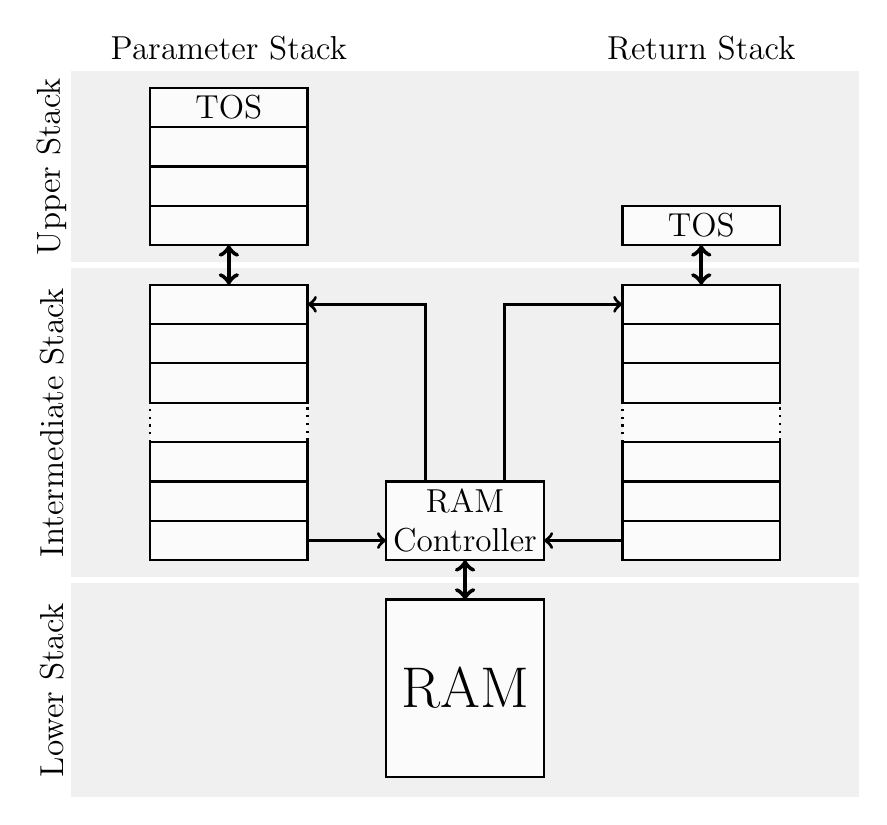
\begin{tikzpicture}

        %Lower stack
        \draw [gray!12, fill=gray!12](0.5,0)   rectangle (10.5,2.7);
        \node [rotate=90] at (0.25,1.35) {\large{Lower Stack}};

        %Intermediate stack
        \draw [gray!12, fill=gray!12](0.5,2.8) rectangle (10.5,6.7);
        \node [rotate=90] at (0.25,4.75) {\large{Intermediate Stack}};

        %Upper stack
        \draw [gray!12, fill=gray!12](0.5,6.8) rectangle (10.5,9.2);
        \node [rotate=90] at (0.25,8) {\large{Upper Stack}};

        %Parameter stack
        \draw [thick, fill=gray!3]        (1.5,7)   rectangle (3.5,7.5);
        \draw [thick, fill=gray!3]        (1.5,7.5) rectangle (3.5,8);
        \draw [thick, fill=gray!3]        (1.5,8)   rectangle (3.5,8.5);
        \draw [thick, fill=gray!3]        (1.5,8.5) rectangle (3.5,9);
        \node at (2.5,8.75) {\large{TOS}};
        \node at (2.5,9.5) {\large{Parameter Stack}};
        \draw [ultra thick, <->] (2.5,7) -- (2.5,6.5);
        \draw [thick, fill=gray!3, dotted](1.5,4.5) rectangle (3.5,5);
        \draw [thick, fill=gray!3]        (1.5,3)   rectangle (3.5,3.5);
        \draw [thick, fill=gray!3]        (1.5,3.5) rectangle (3.5,4);
        \draw [thick, fill=gray!3]        (1.5,4)   rectangle (3.5,4.5);
        \draw [thick, fill=gray!3]        (1.5,5)   rectangle (3.5,5.5);
        \draw [thick, fill=gray!3]        (1.5,5.5) rectangle (3.5,6);
        \draw [thick, fill=gray!3]        (1.5,6)   rectangle (3.5,6.5);          
        \draw [very thick, ->]            (3.5,3.25) --  (4.5,3.25);
        \draw [very thick, <-]            (3.5,6.25) --  (5,6.25) -- (5,4);
        
        %Return stack
        \draw [thick, fill=gray!3]        (7.5,7)   rectangle (9.5,7.5);
        \node at (8.5,7.25) {\large{TOS}};
        \node at (8.5,9.5) {\large{Return Stack}};
        \draw [ultra thick, <->] (8.5,7) -- (8.5,6.5);
        \draw [thick, fill=gray!3, dotted](7.5,4.5) rectangle (9.5,5);
        \draw [thick, fill=gray!3]        (7.5,3)   rectangle (9.5,3.5);
        \draw [thick, fill=gray!3]        (7.5,3.5) rectangle (9.5,4);
        \draw [thick, fill=gray!3]        (7.5,4)   rectangle (9.5,4.5);
        \draw [thick, fill=gray!3]        (7.5,5)   rectangle (9.5,5.5);
        \draw [thick, fill=gray!3]        (7.5,5.5) rectangle (9.5,6);
        \draw [thick, fill=gray!3]        (7.5,6)   rectangle (9.5,6.5);          
        \draw [very thick, ->]            (7.5,3.25) --  (6.5,3.25);
        \draw [very thick, <-]            (7.5,6.25) --  (6,6.25) -- (6,4);
     
        %RAM
        \draw [thick, fill=gray!3] (4.5,0.25) rectangle (6.5,2.5);
        \node at (5.5,1.375) {\huge{RAM}};
        %RAM controller
        \draw [thick, fill=gray!3] (4.5,3)   rectangle (6.5,4);
        \node at (5.5,3.5) {
          \begin{minipage}[c]{10em}
            \begin{center}
              \large{RAM}\\
              \large{Controller}
            \end{center}
        \end{minipage}};
        \draw [ultra thick, <->] (5.5,3) --  (5.5,2.5);
        
       \end{tikzpicture}
    }
  }
  \caption{Stack Architecture}
  \label{stacks:fig}
  \end{center}
\end{figure}

\subsection{Parameter Stack}
\label{stacks:ps}

The \glslink{us}{upper} \gls{ps} holds the four topmost data entries.
Its purpose is to perform stack and \gls{alu} operations
(see \secref{opcodes:stack} and \secref{opcodes:alu}).
When the capacity of the \gls{us} is exceeded, older data entries are shifted
to the \gls{is}.

The \gls{is} serves as a buffer between the \gls{us} and the \gls{ls}, which resides
in \gls{ram}. The purpose of the \gls{is} is to minimize \gls{ram} traffic to and
from the \gls{ls}.
Push operations to the \gls{is} are only propagated to the \gls{ls} when the buffer
capacity is exceeded. Pull operations are only propagated when the \gls{is} is empty.
\Gls{stack} fluctuations within the \gls{is}'s capacity are not visible to the \gls{ls}.

The \gls{ls} is a region of the \gls{ram}, which is managed by a memory controller
that is shared by the \gls{ps} and the \gls{rs}. Within the RAM, both stacks will
grow towards each other. Moving cell content from one stack to the other (\texttt{>R} 
or \texttt{R>}) will never lead to a stack overflow. 

\subsection{Return Stack Stack}
\label{stacks:ps}

The \gls{us} of the \gls{ps} has the capacity of one \gls{cell}. The \gls{is} and
\gls{ls} are identical to the ones of the \gls{ps}.


%--------------------
% Reset, IRQs, and exceptions
%--------------------
%###############################################################################
%# N1 - Manual - Reset, Exceptions, and Interrupts                             #
%###############################################################################
%#    Copyright 2018 - 2019 Dirk Heisswolf                                     #
%#    This file is part of the N1 project.                                     #
%#                                                                             #
%#    N1 is free software: you can redistribute it and/or modify               #
%#    it under the terms of the GNU General Public License as published by     #
%#    the Free Software Foundation, either version 3 of the License, or        #
%#    (at your option) any later version.                                      #
%#                                                                             #
%#    N1 is distributed in the hope that it will be useful,                    #
%#    but WITHOUT ANY WARRANTY; without even the implied warranty of           #
%#    MERCHANTABILITY or FITNESS FOR A PARTICULAR PURPOSE.  See the            #
%#    GNU General Public License for more details.                             #
%#                                                                             #
%#    You should have received a copy of the GNU General Public License        #
%#    along with N1.  If not, see <http://www.gnu.org/licenses/>.              #
%###############################################################################
%# Version History:                                                            #
%#   March 4, 2019                                                             #
%#      - Initial release                                                      #
%###############################################################################

\section{Reset, Exceptions, and Interrupts}
\label{reset}

There are three hardware mechanisms in the N1 processor, which can stop the ongoing
program flow in order to react to an urgent hardware condition:
Reset, Exceptions and Interrupts.

\subsection{Reset}
\label{reset:rst}
A reset puts the entire sequential logic of the N1 into a defined initial state.
The \gls{ps} and the \gls{rs} become cleared and
the \hyperref[opcodes:freg:tc]{Throw Code register (TC)} is set to \texttt{0x0000} (see \tabref{reset:tc}).
After every reset, program execution will begin at address \texttt{0x0000}.
Any context of the previous program flow is lost.
Resets are generated by the system's hardware and occur at least once during power-up.

\subsection{Exceptions}
\label{reset:excpt}
Exceptions are a mechanism to handle error conditions. The are thrown either by hardware or software.
There are five error conditions, which are detected by the N1 hardware:
\begin{description}[style=nextline]
\item[\Gls{ps} overflow]
  A \gls{ps} overflow occurs when the capacity of the lower stack's RAM is exceeded
\item[\Gls{rs} stack underflow]
  A \gls{ps} underflow occurs when an instruction requires more arguments than
  available on the \gls{stack} and when a stack instruction would result in non-continuous filling
  of the stack.
\item[\Gls{rs} overflow]
  A \gls{rs} overflow occurs when the capacity of the lower stack's RAM is exceeded
\item[\Gls{rs} underflow]
  A \gls{rs} underflow occurs when an instruction requires more arguments than
  available on the \gls{rs}.
\item[Address out of range]
  This error condition indicates a memory access to a restricted address. This can either
  be caused by an instruction fetch or a data access
%\item[Undefined word]
%  This error condition is triggered whenever an undefined \gls{opcode} is executed or an
%  unimplemented \gls{freg} is accessed.
\end{description}

Any other error condition must be detected by software and thrown by writing to the
\hyperref[opcodes:freg:tc]{Throw Code register (TC)}.
Whenever an exception is thrown, the N1 processor keeps the associated \gls{tc}
(see \tabref{reset:tc} in the \hyperref[opcodes:freg:tc]{Throw Code register (TC)}.
In case of a \gls{ps} overflow or a \gls{rs} overflow, both stacks will be cleared.
Otherwise, the \gls{rs} and the lower content of the \gls{ps} will be kept,
allowing the \gls{excpt} to be caught by software.
The N1 processor will will then continue with a call to address \texttt{0x0000}.
%Exceptions can be triggered by software (see \secref{opcodes:freg:tc}).

The \glspl{tc} listed in \tabref{reset:tc} comply with the exception word set of
the ANS Forth standard~\cite{dpans94}.

\begingroup
\setlength{\LTleft}{-20cm plus -1fill}
\setlength{\LTright}{\LTleft}
\begin{center}
  \rowcolors{1}{gray!12}{white}                                         %set alternating row color
  \begin{longtable}{|c|l|}
    \rowcolor{white}
    \caption{Throw codes}
    \label{reset:tc} \\
    %Header
    \hline                                     
    \rowcolor{gray!25}
    \multicolumn{1}{|c|}{\textbf{\rule{0pt}{2.5ex}Throw Code}}     &  
    \multicolumn{1}{c|}{\textbf{\rule{0pt}{2.5ex}Condition}}\\
    \hline
    \endhead                               
    %Footers
    \hline
    \rowcolor{white}
    \multicolumn{2}{r}{\tiny{...continued}} \\
    \endfoot
    \hline
    \endlastfoot

    %Reset
    \texttt{0x0000} (0)                 &    
    Reset (no exception)                \\* \hline

    \texttt{0x0001} (1)                 &    
    No exception                        \\* \hline
       
    %Parameter stack overflow
    \texttt{0xFFFD} (-3)                &    
    Parameter stack overflow            \\* \hline

    %Parameter stack underflow
    \texttt{0xFFFC} (-4)                &    
      Parameter stack underflow         \\* \hline

    % stack overflow
    \texttt{0xFFFB} (-5)                &    
    Parameter stack overflow            \\* \hline

    %Parameter stack underflow
    \texttt{0xFFFA} (-6)                &    
    Parameter stack underflow           \\* \hline

    %Invalid memory address
    \texttt{0xFFF7} (-9)                &    
    Invalid memory address              \\* \hline

%    %Undefined word
%    \texttt{0xFFF3} (-13)                &    
%    Undefined word                       \\* \hline

  \end{longtable}
\end{center}  
\endgroup

\noindent
%The five hardware exceptions can be easily complemented by user defined software exceptions.
%Software exceptions can be thrown by pushing a unique \gls{tc} onto the \gls{ps} and performing
%a \gls{jump} to address \texttt{0x0000}.
%Hardware and software exceptions can then be handled by a common exception handler routine.

\subsection{Interrupts}
\label{reset:irq}
interrupts are an optional feature (see \secref{extensions:int})

%Interrupts are service requests which are generated by the peripheral hardware. They cause
%a temporary interruption of the ongoing program flow. 
%When an iterrupt occurs, the program counter is saved to the \gls{rs} and an interrupt service
%routine is executed. The location of the interrupt service routine is determined by the system's
%interrupt controller hardware. Further interrupts are automatically disabled during the execution
%of the interrupt service routine and must be manually reenabled by a control instruction
%(see \tabref{opcodes:ctrl:smpl}) before resuming the interrupted program flow.


%--------------------
% N1 Integration guide
%--------------------
%###############################################################################
%# N1 - Manual - Integration Guide                                             #
%###############################################################################
%#    Copyright 2018 - 2019 Dirk Heisswolf                                     #
%#    This file is part of the N1 project.                                     #
%#                                                                             #
%#    N1 is free software: you can redistribute it and/or modify               #
%#    it under the terms of the GNU General Public License as published by     #
%#    the Free Software Foundation, either version 3 of the License, or        #
%#    (at your option) any later version.                                      #
%#                                                                             #
%#    N1 is distributed in the hope that it will be useful,                    #
%#    but WITHOUT ANY WARRANTY; without even the implied warranty of           #
%#    MERCHANTABILITY or FITNESS FOR A PARTICULAR PURPOSE.  See the            #
%#    GNU General Public License for more details.                             #
%#                                                                             #
%#    You should have received a copy of the GNU General Public License        #
%#    along with N1.  If not, see <http://www.gnu.org/licenses/>.              #
%###############################################################################
%# Version History:                                                            #
%#   March 4, 2019                                                             #
%#      - Initial release                                                      #
%###############################################################################

\section{Integration Guide}
\label{integration}

This section outlines the interfaces and configurations of the N1 processor
for system integration.

\subsection{Integratation Parameters}
\label{integration:params}

The N1 processor supports six \gls{verilog} integration parameters to configure
the design for application specific needs:

\begin{description}[style=nextline]

\item[\texttt{SP\_WIDTH}] Stack pointer width. \\
  This parameter determines the address width of the \gls{ls}.
  Values in the range of 5 to 16 are valid.
  The default value is 12. 
  
\item[\texttt{IPS\_DEPTH}] Depth of the intermediate parameter stack. \\
  This parameter determines the number of \glspl{cell} in the \gls{is} of the \gls{ps}.
  Any value larger than 2 is valid.
  The default value is 8. 
  The purpose of the \gls{is} is to conceal fluctuations in stack usage to the \gls{ls}.
  The optimal value should be derived from the application use case.

\item[\texttt{IRS\_DEPTH}] Depth of the intermediate return stack. \\
  This parameter determines the number of \glspl{cell} in the \gls{is} of the \gls{rs}.
  Any value larger than 2 is valid.
  The default value is 8. 
  The purpose of the \gls{is} is to conceal fluctuations in stack usage to the \gls{ls}.
  The optimal value should be derived from the application use case.

\item[\texttt{PBUS\_AADR\_OFFSET}] Offset for direct \gls{jump} or \gls{call} addressing. \\
  This parameter determines the location of the 32KB window for \glspl{jump} and \glspl{call}
  with \gls{diradr}.
  The default value is \texttt{0x0000}. 

\item[\texttt{PBUS\_MADR\_OFFSET}] Offset for direct data accesses. \\
  This parameter determines the location of the 511B window for memory I/O with \gls{diradr}.
  This window should cover commonly used \gls{forth} variables. The default value is \texttt{0xFFFF}. 

\item[\texttt{PS\_RS\_DIST}] Safety distance between the \gls{ps} and the \gls{rs}. \\
  Recovering from an exception requires some free \gls{stack} space.
  This parameter determines the remaining \gls{stack} space when a \gls{stack} overflow exception is thrown.
  The default value is 22. The optimal value depends on the requirements of the exception handler software.

\end{description}

\subsection{Interfaces}
\label{integration:if}

The N1 processor provides four interfaces which must be connected at system level.
A fifth one (see \secref{integration:if:prb}) is only to be used for verification and debug purposes.

\subsubsection{Clock and Resets}
\label{integration:if:clk}
This interface provides clocks and resets for all sequential logic in the N1 design.

\begin{description}[style=nextline]

\item[\texttt{clk\_i}] Single clock input. \\  
  This clock is used for all interfaces as well as all internal sequential logic.

\item[\texttt{async\_rst\_i}] Asynchronous reset input. \\
  This active high reset input may assert asynchronously, but must deassert synchronously.
  This signal is not required if a synchrounous reset (\texttt{sync\_rst\_i}) is implemented.
  If unused, this input must be tied to \texttt{0}.

\item[\texttt{sync\_rst\_i}] Synchronous reset input. \\
  This active high reset input must assert and deassert synchronously.
  This signal is not required if an asynchrounous reset (\texttt{async\_rst\_i}) is implemented.
  If unused, this input must be tied to \texttt{0}.
 
\end{description}

\subsubsection{Program Bus}
\label{integration:if:pbus}
This interface connects the N1 to the main memory.
All signals comply to the \gls{wb} protocoll~\cite{wishbone}.

\begin{description}[style=nextline]
  
\item[\texttt{pbus\_cyc\_o}] Cycle indicator output. \\
  This output signal corresponds to signal \texttt{CYC\_O} of the Wishbone specification~\cite{wishbone}.

\item[\texttt{pbus\_stb\_o}] Strobe output. \\   
  This output signal corresponds to signal \texttt{STB\_O} of the Wishbone specification~\cite{wishbone}.

\item[\texttt{pbus\_we\_o}]  Write enable output. \\
  This output signal corresponds to signal \texttt{WE\_O} of the Wishbone specification~\cite{wishbone}.

\item[\texttt{pbus\_adr\_o}] Address bus. \\   
  These output signals correspond to bus \texttt{ADR\_O} of the Wishbone specification~\cite{wishbone}.

\item[\texttt{pbus\_dat\_o}] Write data bus. \\    
  These output signals correspond to bus \texttt{DAT\_O} of the Wishbone specification~\cite{wishbone}.

\item[\texttt{pbus\_tga\_cof\_jmp\_o}] Change of flow indicator. \\   
  This output signal corresponds to bus \texttt{TGA\_O} of the Wishbone specification~\cite{wishbone}.
  It indicates, that the current bus access was caused by a \gls{jump} instruction.
  This information may be used to trace the program flow.

\item[\texttt{pbus\_tga\_cof\_cal\_o}] Change of flow indicator. \\   
  This output signal corresponds to bus \texttt{TGA\_O} of the Wishbone specification~\cite{wishbone}.
  It indicates, that the current bus access was caused by either a \gls{call} instruction or an
  interrupt service request.
  This information may be used to trace the program flow.

\item[\texttt{pbus\_tga\_cof\_bra\_o}] Change of flow indicator. \\   
  This output signal corresponds to bus \texttt{TGA\_O} of the Wishbone specification~\cite{wishbone}.
  It indicates, that the current bus access was caused by a \gls{branch} instruction.
  This information may be used to trace the program flow.

\item[\texttt{pbus\_tga\_cof\_eow\_o}] Change of flow indicator. \\   
  This output signal corresponds to bus \texttt{TGA\_O} of the Wishbone specification~\cite{wishbone}.
  It indicates ,that the current bus access was caused by a return from a \gls{call}.
  This information may be used to trace the program flow.

\item[\texttt{pbus\_ack\_i}] Acknowlede input. \\   
  This input signal corresponds to signal \texttt{ACK\_I} of the Wishbone specification~\cite{wishbone}.
  If unused, this input must be tied to \texttt{1}.

\item[\texttt{pbus\_err\_i}] Error indicator input. \\  
  This input signal corresponds to signal \texttt{ERR\_I} of the Wishbone specification~\cite{wishbone}.
  It informs the N1 processor, that the current address exceeds the valid range of the connected
  memory system. 
  If unused, this input must be tied to \texttt{0}.
  
\item[\texttt{pbus\_stall\_i}] Pipeline stall input. \\
  This input signal corresponds to signal \texttt{STALL\_I} of the Wishbone specification~\cite{wishbone}.
  If unused, this input must be tied to \texttt{0}.

\item[\texttt{pbus\_dat\_i}] Read data bus. \\ 
  These input signals correspond to bus \texttt{DAT\_I} of the Wishbone specification~\cite{wishbone}.

\end{description}

\subsubsection{Stack Bus}
\label{integration:if:sbus}
This interface connects the N1 to the stack memory.
It is expected that the \texttt{SP\_WIDTH} parameter (see \secref{integration:params}) matches the
implemented memory size. Therefore no \texttt{ERR\_I} input is needed in this interface.
All signals comply to the \gls{wb} protocoll~\cite{wishbone}.

\begin{description}[style=nextline]

\item[\texttt{sbus\_cyc\_o}] Cycle indicator output. \\
  This output signal corresponds to signal \texttt{CYC\_O} of the Wishbone specification~\cite{wishbone}.

\item[\texttt{sbus\_stb\_o}] Strobe output. \\   
  This output signal corresponds to signal \texttt{STB\_O} of the Wishbone specification~\cite{wishbone}.

\item[\texttt{sbus\_we\_o}]  Write enable output. \\
  This output signal corresponds to signal \texttt{WE\_O} of the Wishbone specification~\cite{wishbone}.

\item[\texttt{sbus\_adr\_o}] Address bus. \\   
  These output signals correspond to bus \texttt{ADR\_O} of the Wishbone specification~\cite{wishbone}.

\item[\texttt{sbus\_dat\_o}] Write data bus. \\    
  These output signals correspond to bus \texttt{DAT\_O} of the Wishbone specification~\cite{wishbone}.

\item[\texttt{sbus\_tga\_ps\_o}] \Gls{ps} access indicator. \\   
  These output signals correspond to bus \texttt{TGA\_O} of the Wishbone specification~\cite{wishbone}.
  It indicates, that the current bus access is associated with the \gls{ps}.

\item[\texttt{sbus\_tga\_rs\_o}] \Gls{rs} access indicator. \\   
  These output signals correspond to bus \texttt{TGA\_O} of the Wishbone specification~\cite{wishbone}.
  It indicates, that the current bus access is associated with the \gls{rs}.
  
\item[\texttt{sbus\_ack\_i}] Acknowlede input. \\   
  This input signal corresponds to signal \texttt{ACK\_I} of the Wishbone specification~\cite{wishbone}.
  If unused, this input must be tied to \texttt{1}.

\item[\texttt{sbus\_stall\_i}] Pipeline stall input. \\
  This input signal corresponds to signal \texttt{STALL\_I} of the Wishbone specification~\cite{wishbone}.
  If unused, this input must be tied to \texttt{0}.

\item[\texttt{sbus\_dat\_i}] Read data bus. \\ 
  These input signals correspond to bus \texttt{DAT\_I} of the Wishbone specification~\cite{wishbone}.

\end{description}

\subsubsection{Interrupt Interface}
\label{integration:if:irq}
This interface connects an optional interrupt controller to the N1 processor. 


\begin{description}[style=nextline]

\item[\texttt{irq\_ack\_o}] Interrupt acknowledge. \\
  This output signal asserts for one clock cycle, whenever the current interrupt is serviced.
  It may be used for automatic flag clearing.

\item[\texttt{irq\_req\_i}] Interrupt request. \\
  Any non-zero value driven to this bus interface is interpreted as interrupt request.
  The value determines the start address of the interrupt service routine that is to be executed by the
  N1 processor. This bus must be tied to \texttt{0x0000} if no interrupt controller is connected.
  
\end{description}

\subsubsection{Probe Signals}
\label{integration:if:prb}
This interface propagates all internal states of the N1 processor to the outside.
It is solely intended for verification and debug purposes and should be left unconnected for system integration.
The signals in this interface are specific to the internal implementation of the N1 processor and may change
with every revision.

\subsection{Target Specific Design Files}
\label{integration:ifs}
All adder and multiplier logic of the N1 design ls located in a single \gls{verilog} module called \texttt{N1\_dsp}.
A synthesizable implementation of this module, can be found in the file \texttt{rtl/verolog/N1\_dsp\_synth.v}.
If desired, this file can be replaced by one containing a alternative implementation of the \texttt{N1\_dsp} module.
An example is given in in the file \texttt{rtl/verolog/N1\_dsp\_iCE40UP5K.v}.
It contains a custom implementation for Lattice iCE40 FPGAs, utilizing four hard instantiated \texttt{SB\_MAC16}
macro cells.



%--------------------
% N1 Architecture
%--------------------
%%###############################################################################
%# N1 - Manual - Architecture Description                                      #
%###############################################################################
%#    Copyright 2018 - 2022 Dirk Heisswolf                                     #
%#    This file is part of the N1 project.                                     #
%#                                                                             #
%#    N1 is free software: you can redistribute it and/or modify               #
%#    it under the terms of the GNU General Public License as published by     #
%#    the Free Software Foundation, either version 3 of the License, or        #
%#    (at your option) any later version.                                      #
%#                                                                             #
%#    N1 is distributed in the hope that it will be useful,                    #
%#    but WITHOUT ANY WARRANTY; without even the implied warranty of           #
%#    MERCHANTABILITY or FITNESS FOR A PARTICULAR PURPOSE.  See the            #
%#    GNU General Public License for more details.                             #
%#                                                                             #
%#    You should have received a copy of the GNU General Public License        #
%#    along with N1.  If not, see <http://www.gnu.org/licenses/>.              #
%###############################################################################
%# Version History:                                                            #
%#   November 11, 2022                                                         #
%#      - Initial release                                                      #
%###############################################################################

\section{Architecture Description}
\label{architecture}

The following sections provide some descriptions of the internal N1 design.


\subsection{Design Principles}
\label{architecture:principles}

The RTL implementation of the N1 follows a number of design principles which are captured in following sections. 

\subsubsection{Naming Convention of Interface Signals}
\label{architecture:principles:naming}

For all signals, which do not implement a common standard (e.g. \gls{wb}),
the following signal naming rules are used throughout the design:
\begin{itemize}

\item   
All interface signals of a point-to-point connection, contain a mnemonic of the sending and the receiving block in its prefix.
The format of the prefix is: \\
\emph{\textless sender mnemonic\textgreater}\texttt{2}\emph{\textless receiver mnemonic\textgreater }\texttt{\_}\dots \\
Example: \texttt{\underline{fc2ir\_}capture}

\item   
Control signals which represent a request, end with a verb in imperative form. \\
Example: \texttt{fc2ir\_\underline{expend}}

\item   
Status signals represening a busy indicator, have the postfix \dots\texttt{\_bsy} \\
Example: \texttt{prs2fc\_\underline{bsy}}

\item   
If a signal is connected to the interface of a module, a further postfix is added to indicate the signal direction:
  \begin{itemize}
    \item   
    Input signals: \dots\texttt{\_i} \\
    \item   
    Output signals: \dots\texttt{\_o} \\
  \end{itemize}
Example: \texttt{prs2fc\_bsy\underline{\_o}}
  
\item   
Names of signals which are only used within one design block are kept short and don't follow a particular naming convention.

\end{itemize}

\subsubsection{Handshaking}
\label{architecture:principles:handshakes}

A high signal level of a contol signal is interpreted a request by the receiving design block.
The request is expected to be immediately accepted by the receiver and processed in the next clock cycle,
unless the receiver provides a busy indicator (\dots\texttt{\_bsy}).
In this case the request in only accepted if the busy indicator was deasserted in the cycle, in which the request is made.

\subsubsection{Instruction Boundaries}
\label{architecture:principles:ibounds}

The \hyperref[architecture:comp:ir]{instruction register} always contains the instruction which is currently in execution.
Before the execution of an instruction can ce concluded and the next one can begin, the fillowing conditions must be fulfilled:
\begin{itemize}

\item   
The program bus must be available - TBD
  
\item   
The parameter and the return stack must be available - TBD
  
\end{itemize}

\subsection{Common Internal Interfaces}
\label{architecture:interfaces}

The subblocks in the N1 design use common interfaces for common functionality. These interfaces follow the
\hyperref[architecture:principles:naming]{naming conventions} and \hyperref[architecture:principles:handshakes]{handshaking concept} 
described in \secref{architecture:principles}.

\subsubsection{Stack Interface}
\label{architecture:interfaces:stack}

All stacks are controlled using the following interface:
\begin{description}[style=nextline]

\item[\emph{\textless stack name\textgreater}\texttt{\_clear\_o}/\texttt{\_i} {\scriptsize (controller $\rightarrow$ stack)}]
  Request to clear the stack.
  
\item[\emph{\textless stack name\textgreater}\texttt{\_clear\_bsy\_i}/\texttt{\_o} {\scriptsize (controller $\leftarrow$ stack)}]
  Busy indicator. \\
  The stack will be cleared if \emph{\textless stack name\textgreater}\texttt{\_clear\_i} is asseeted while \\
  \emph{\textless stack name\textgreater}\texttt{\_clear\_bsy\_o} is deasserted.

\item[\emph{\textless stack name\textgreater}\texttt{\_push\_o}/\texttt{\_i} {\scriptsize (controller $\rightarrow$ stack)}]
  Request to push a data word onto the stack.

\item[\emph{\textless stack name\textgreater}\texttt{\_push\_data\_o}/\texttt{\_i[15:0]} {\scriptsize (controller $\rightarrow$ stack)}]
  Data word to be pushed onto the stack. \\
  The data word must be supplied in the same clock cycle as the request.

\item[\emph{\textless stack name\textgreater}\texttt{\_push\_bsy\_i}/\texttt{\_o} {\scriptsize (controller $\leftarrow$ stack)}]
  Busy indicator. \\
  \emph{\textless stack name\textgreater}\texttt{\_push\_data\_i} will be pushed onto the stack if
  \emph{\textless stack name\textgreater}\texttt{\_push\_i} is asserted while
  \emph{\textless stack name\textgreater}\texttt{\_push\_bsy\_o} and 
  \emph{\textless stack name\textgreater}\texttt{\_push\_of\_o} are deasserted.
  
\item[\emph{\textless stack name\textgreater}\texttt{\_push\_of\_i}/\texttt{\_o} {\scriptsize (controller $\leftarrow$ stack)}]
  Overflow indicator. \\
  \emph{\textless stack name\textgreater}\texttt{\_push\_of\_o} is asserted when the stack is full and a new push request would cause an overflow.

\item[\emph{\textless stack name\textgreater}\texttt{\_pull\_o}/\texttt{\_i} {\scriptsize (controller $\rightarrow$ stack)}]
  Request to pull a data word from the stack.

\item[\emph{\textless stack name\textgreater}\texttt{\_pull\_data\_i}/\texttt{\_o[15:0]} {\scriptsize (controller $\leftarrow$ stack)}]
  Data word to be pulled from the stack. If the stack is not empty \\
  (\emph{\textless stack name\textgreater}\texttt{\_pull\_uf\_o} deasserted)
  and ready for a pull operation \\
  (\emph{\textless stack name\textgreater}\texttt{\_pull\_bsy\_o} deasserted),
  then \emph{\textless stack name\textgreater}\texttt{\_pull\_data\_o} always shows the data at the top of the stack.

\item[\emph{\textless stack name\textgreater}\texttt{\_pull\_bsy\_i}/\texttt{\_o} {\scriptsize (controller $\leftarrow$ stack)}]
  Busy indicator. \\
  The data at the top of the stack will be removed if
  \emph{\textless stack name\textgreater}\texttt{\_pull\_i} is asserted while
  \emph{\textless stack name\textgreater}\texttt{\_pull\_bsy\_o} and 
  \emph{\textless stack name\textgreater}\texttt{\_pull\_uf\_o} are deasserted.

\item[\emph{\textless stack name\textgreater}\texttt{\_pull\_uf\_i}/\texttt{\_o} {\scriptsize (controller $\leftarrow$ stack)}]
  Underflow indicator. \\
  \emph{\textless stack name\textgreater}\texttt{\_pull\_uf\_o} is asserted when the stack is empty and a new pull request would cause an underflow.

\end{description}

\subsubsection{Memory Interface}
\label{architecture:interfaces:memory}

Memories are connected through the following interface:
\begin{description}[style=nextline]

\item[\emph{\textless memory name\textgreater}\texttt{\_addr\_o}/\texttt{\_i[$n$-1:0]} {\scriptsize (controller $\rightarrow$ memory)}]
  Memory address.
  
\item[\emph{\textless memory name\textgreater}\texttt{\_raddr\_o}/\texttt{\_i[$n$-1:0]} {\scriptsize (controller $\rightarrow$ memory)}]
  Memory address for read accesses to dual ported RAMs.
  
\item[\emph{\textless memory name\textgreater}\texttt{\_waddr\_o}/\texttt{\_i[$n$-1:0]} {\scriptsize (controller $\rightarrow$ memory)}]
  Memory address for write accesses to dual ported RAMs.
  
\item[\emph{\textless memory name\textgreater}\texttt{\_write\_o}/\texttt{\_i} {\scriptsize (controller $\rightarrow$ memory)}]
  Write request.
  
\item[\emph{\textless memory name\textgreater}\texttt{\_read\_o}/\texttt{\_i} {\scriptsize (controller $\rightarrow$ memory)}]
  Read request.

\item[\emph{\textless memory name\textgreater}\texttt{\_write\_bsy\_i}/\texttt{\_o} {\scriptsize (controller $\leftarrow$ memory)}]
  Busy indicator. \\
  A write request is valid if
  \emph{\textless memory name\textgreater}\texttt{\_write\_i} is asserted while \\
  \emph{\textless memory name\textgreater}\texttt{\_write\_bsy\_o} is deasserted.

\item[\emph{\textless memory name\textgreater}\texttt{\_read\_bsy\_i}/\texttt{\_o} {\scriptsize (controller $\leftarrow$ memory)}]
  Busy indicator. \\
  A read request is valid if
  \emph{\textless memory name\textgreater}\texttt{\_read\_i} is asserted while \\
  \emph{\textless memory name\textgreater}\texttt{\_read\_bsy\_o} is deasserted.
  
\item[\emph{\textless memory name\textgreater}\texttt{\_wdata\_o}/\texttt{\_i[15:0]} {\scriptsize (controller $\rightarrow$ memory)}]
  Write data. \\
  Write data must be driven in the same clock cycle as the request.
  
\item[\emph{\textless memory name\textgreater}\texttt{\_rdata\_i}/\texttt{\_o[15:0]} {\scriptsize (controller $\leftarrow$ memory)}]
  Read data. \\
  Read data must be captured one clock cyle after a valid request has been captured.

\end{description}

\subsection{Instruction Execution Cycle}
\label{architecture:excyc}

The execution cycle of the N1 processor characterized by the following design components:
\begin{description}[style=nextline]

\item[\textbf{Program Counter}]
A 16-bit register, which contains the memory location on the next instruction to be executed.  
It is implemented within the \hyperref[architecture:comp:dsp]{DSP Block}.

\item[\textbf{Address Bus}]
The address output of the \hyperref[integration:if:pbus]{Program Bus (\texttt{pbus\_adr\_o})}.

\item[\textbf{Read Data Bus}]
The read data input of the \hyperref[integration:if:pbus]{Program Bus (\texttt{pbus\_dat\_i})}

\item[\textbf{Instruction Register}]
A 16-bit register holding the opcode of the instruction, which is currently executed (see \secref{architecture:comp:ir}).

\item[\textbf{Instruction Stash Register}]
A 16-bit register to temoprarily store an upcoming opcode. (see \secref{architecture:comp:ir}).

\end{description}

The following sections show the timing relation of these design components in different execution scenarios.


\subsubsection{Plain Linear Execution}
\label{architecture:excyc:linear}

Most of of the  N1 instructuins are executed in a single clock cycle.
\figref{architecture:excyc:linear:fig} the typical linear execution flow of single cycle instructions.

The opcode stored in the instruction register determines which instruction is currently being executed.
The program counter points to the address of the next instruction.
The address bus is unregistered and always runs one clock cycle ahead of the program counter. 
The resulting data on the read data bus is captured by the instruction register in the next clock cycle.

    
\begin{figure}[!h]
  \begin{center}
  \makebox[\textwidth][c]{
  \scalebox{1} {
      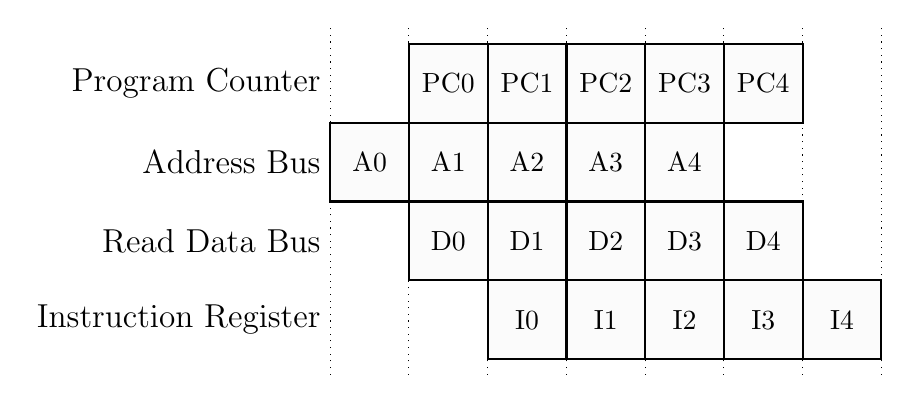
\begin{tikzpicture}

        %Lines
        \draw [dotted] (0,0.3) -- (0,4.7);
        \draw [dotted] (1,0.3) -- (1,4.7);
        \draw [dotted] (2,0.3) -- (2,4.7);
        \draw [dotted] (3,0.3) -- (3,4.7);
        \draw [dotted] (4,0.3) -- (4,4.7);
        \draw [dotted] (5,0.3) -- (5,4.7);
        \draw [dotted] (6,0.3) -- (6,4.7);
        \draw [dotted] (7,0.3) -- (7,4.7);

        %Program counter
        \node  [left] at (0,4) {\large{Program Counter}};
        \draw [thick, fill=gray!3] (1,4.5) rectangle (2,3.5);
        \node at (1.5,4)  {PC0};
        \draw [thick, fill=gray!3] (2,4.5) rectangle (3,3.5);
        \node at (2.5,4)  {PC1};
        \draw [thick, fill=gray!3] (3,4.5) rectangle (4,3.5);
        \node at (3.5,4)  {PC2};
        \draw [thick, fill=gray!3] (4,4.5) rectangle (5,3.5);
        \node at (4.5,4)  {PC3};
        \draw [thick, fill=gray!3] (5,4.5) rectangle (6,3.5);
        \node at (5.5,4)  {PC4};
        
        %Address bus
        \node [left] at (0,3) {\large{Address Bus}};
        \draw [thick, fill=gray!3] (0,3.5) rectangle (1,2.5);
        \node at (0.5,3)  {A0};
        \draw [thick, fill=gray!3] (1,3.5) rectangle (2,2.5);
        \node at (1.5,3)  {A1};
        \draw [thick, fill=gray!3] (2,3.5) rectangle (3,2.5);
        \node at (2.5,3)  {A2};
        \draw [thick, fill=gray!3] (3,3.5) rectangle (4,2.5);
        \node at (3.5,3)  {A3};
        \draw [thick, fill=gray!3] (4,3.5) rectangle (5,2.5);
        \node at (4.5,3)  {A4};

        %Read data bus
        \node [left] at (0,2) {\large{Read Data Bus}};
        \draw [thick, fill=gray!3] (1,2.5) rectangle (2,1.5);
        \node at (1.5,2)  {D0};
        \draw [thick, fill=gray!3] (2,2.5) rectangle (3,1.5);
        \node at (2.5,2)  {D1};
        \draw [thick, fill=gray!3] (3,2.5) rectangle (4,1.5);
        \node at (3.5,2)  {D2};
        \draw [thick, fill=gray!3] (4,2.5) rectangle (5,1.5);
        \node at (4.5,2)  {D3};
        \draw [thick, fill=gray!3] (5,2.5) rectangle (6,1.5);
        \node at (5.5,2)  {D4};

        %Instruction register
        \node [left] at (0,1) {\large{Instruction Register}};
        \draw [thick, fill=gray!3] (2,1.5) rectangle (3,0.5);
        \node at (2.5,1)  {I0};
        \draw [thick, fill=gray!3] (3,1.5) rectangle (4,0.5);
        \node at (3.5,1)  {I1};
        \draw [thick, fill=gray!3] (4,1.5) rectangle (5,0.5);
        \node at (4.5,1)  {I2};
        \draw [thick, fill=gray!3] (5,1.5) rectangle (6,0.5);
        \node at (5.5,1)  {I3};
        \draw [thick, fill=gray!3] (6,1.5) rectangle (7,0.5);
        \node at (6.5,1)  {I4};

      \end{tikzpicture}
    }
  }
  \caption{Plain Linear Execution}
  \label{architecture:excyc:linear:fig}
  \end{center}
\end{figure}


\subsubsection{Execution of Extended Instructions}
\label{architecture:excyc:extended}

In some cases the execution of an instruction can span multiple cycles (i.e. \hyperref[opcodes:ctrl]{non-concurrent control instructions}
or any instruction waiting for a blocked stack access). 
\figref{architecture:excyc:extended:fig} illustrates the timing in these scenarios.

Whenever an opcode needs to be captured from the read data bus, but the instruction register is blocked by an instruction spaning multiple cycles,
The incoming opcode needs to be temourarely stashed away in a separate register.
When the execution of the ongoing instruction is finished, the stashed opcode is moved into the instruction register.

\begin{figure}[!h]
  \begin{center}
  \makebox[\textwidth][c]{
  \scalebox{1} {
      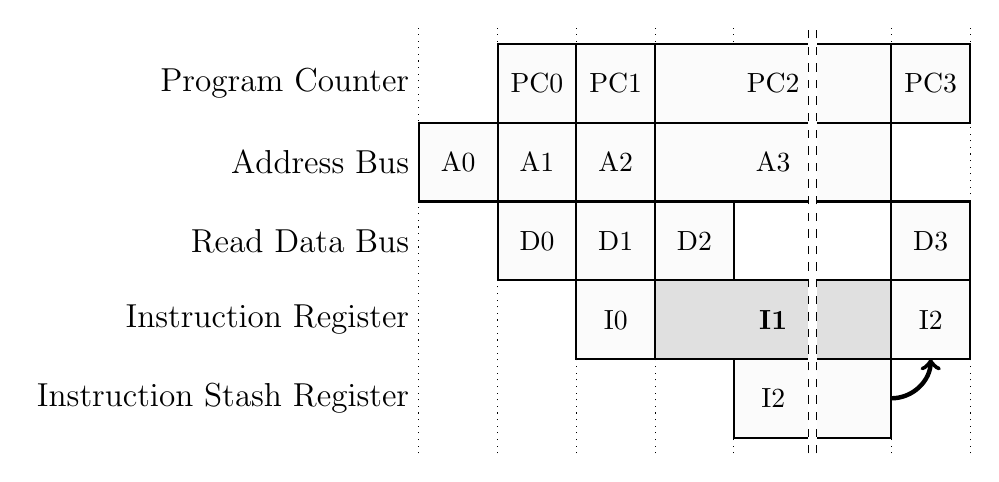
\begin{tikzpicture}

        %Lines
        \draw [dotted] (0,-0.7) -- (0,4.7);
        \draw [dotted] (1,-0.7) -- (1,4.7);
        \draw [dotted] (2,-0.7) -- (2,4.7);
        \draw [dotted] (3,-0.7) -- (3,4.7);
        \draw [dotted] (4,-0.7) -- (4,4.7);
        %\draw [dotted] (5,-0.7) -- (5,4.7);
        \draw [dotted] (6,-0.7) -- (6,4.7);
        \draw [dotted] (7,-0.7) -- (7,4.7);

        %Program counter
        \node  [left] at (0,4) {\large{Program Counter}};
        \draw [thick, fill=gray!3] (1,4.5) rectangle (2,3.5);
        \node at (1.5,4)  {PC0};
        \draw [thick, fill=gray!3] (2,4.5) rectangle (3,3.5);
        \node at (2.5,4)  {PC1};
        \draw [thick, fill=gray!3] (3,4.5) rectangle (6,3.5);
        \node  at (4.5,4)  {PC2};
        \draw [thick, fill=gray!3] (6,4.5) rectangle (7,3.5);
        \node at (6.5,4)  {PC3};
        
        %Address bus
        \node [left] at (0,3) {\large{Address Bus}};
        \draw [thick, fill=gray!3] (0,3.5) rectangle (1,2.5);
        \node at (0.5,3)  {A0};
        \draw [thick, fill=gray!3] (1,3.5) rectangle (2,2.5);
        \node at (1.5,3)  {A1};
        \draw [thick, fill=gray!3] (2,3.5) rectangle (3,2.5);
        \node at (2.5,3)  {A2};
        \draw [thick, fill=gray!3] (3,3.5) rectangle (6,2.5);
        \node at (4.5,3)  {A3};

        %Read data bus
        \node [left] at (0,2) {\large{Read Data Bus}};
        \draw [thick, fill=gray!3] (1,2.5) rectangle (2,1.5);
        \node at (1.5,2)  {D0};
        \draw [thick, fill=gray!3] (2,2.5) rectangle (3,1.5);
        \node at (2.5,2)  {D1};
        \draw [thick, fill=gray!3] (3,2.5) rectangle (4,1.5);
        \node at (3.5,2)  {D2};
        \draw [thick, fill=gray!3] (6,2.5) rectangle (7,1.5);
        \node at (6.5,2)  {D3};

        %Instruction register
        \node [left] at (0,1) {\large{Instruction Register}};
        \draw [thick, fill=gray!3] (2,1.5) rectangle (3,0.5);
        \node at (2.5,1)  {I0};
        \draw [thick, fill=gray!24] (3,1.5) rectangle (6,0.5);
        \node at (4.5,1)  {\textbf{I1}};
        \draw [thick, fill=gray!3] (6,1.5) rectangle (7,0.5);
        \node at (6.5,1)  {I2};

        %Instruction stashregister
        \node [left] at (0,0) {\large{Instruction Stash Register}};
        \draw [thick, fill=gray!3] (4,0.5) rectangle (6,-0.5);
        \node at (4.5,0)  {I2};
        %\draw [ultra thick, ->]  (5,0) -- (5.5,0) -- (5.5,0.5);
        \draw [ultra thick, ->] (6,0) arc (270:360:0.5) ;

        %Gap
        %\draw [dotted] (5,-0.7) -- (5,4.7);
        \draw [fill=white, white] (4.95,-0.7) rectangle (5.05,4.7);
        \draw [dashed] (4.95,-0.7) -- (4.95,4.7);
        \draw [dashed] (5.05,-0.7) -- (5.05,4.7);

        
      \end{tikzpicture}
    }
  }
  \caption{Execution of an Extended Instruction}
  \label{architecture:excyc:extended:fig}
  \end{center}
\end{figure}


\subsubsection{Execution of Memory Access Instructions}
\label{architecture:excyc:mem}

A special case of multi-cycle instructions are \hyperref[opcodes:memacc]{memory access instructions}.
These instructions perform their memory acesses on the program bus.
\figref{architecture:excyc:mem:fig} illustrates how opcode fetches and data accesses are interleaved.

\begin{figure}[!h]
  \begin{center}
  \makebox[\textwidth][c]{
  \scalebox{1} {
      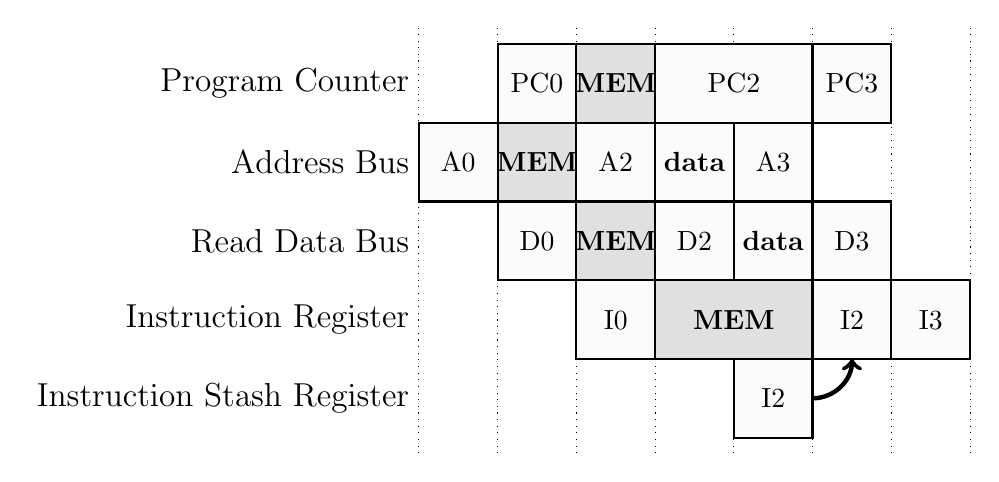
\begin{tikzpicture}

        %Lines
        \draw [dotted] (0,-0.7) -- (0,4.7);
        \draw [dotted] (1,-0.7) -- (1,4.7);
        \draw [dotted] (2,-0.7) -- (2,4.7);
        \draw [dotted] (3,-0.7) -- (3,4.7);
        \draw [dotted] (4,-0.7) -- (4,4.7);
        \draw [dotted] (5,-0.7) -- (5,4.7);
        \draw [dotted] (6,-0.7) -- (6,4.7);
        \draw [dotted] (7,-0.7) -- (7,4.7);

        %Program counter
        \node  [left] at (0,4) {\large{Program Counter}};
        \draw [thick, fill=gray!3] (1,4.5) rectangle (2,3.5);
        \node at (1.5,4)  {PC0};
        \draw [thick, fill=gray!24] (2,4.5) rectangle (3,3.5);
        \node at (2.5,4)  {\textbf{MEM}};
        \draw [thick, fill=gray!3] (3,4.5) rectangle (5,3.5);
        \node  at (4,4)  {PC2};
        \draw [thick, fill=gray!3] (5,4.5) rectangle (6,3.5);
        \node at (5.5,4)  {PC3};
        
        %Address bus
        \node [left] at (0,3) {\large{Address Bus}};
        \draw [thick, fill=gray!3] (0,3.5) rectangle (1,2.5);
        \node at (0.5,3)  {A0};
        \draw [thick, fill=gray!24] (1,3.5) rectangle (2,2.5);
        \node at (1.5,3)  {\textbf{MEM}};
        \draw [thick, fill=gray!3] (2,3.5) rectangle (3,2.5);
        \node at (2.5,3)  {A2};
        \draw [thick, fill=gray!3] (3,3.5) rectangle (4,2.5);
        \node at (3.5,3)  {\textbf{data}};
        \draw [thick, fill=gray!3] (4,3.5) rectangle (5,2.5);
        \node at (4.5,3)  {A3};

        %Read data bus
        \node [left] at (0,2) {\large{Read Data Bus}};
        \draw [thick, fill=gray!3] (1,2.5) rectangle (2,1.5);
        \node at (1.5,2)  {D0};
        \draw [thick, fill=gray!24] (2,2.5) rectangle (3,1.5);
        \node at (2.5,2)  {\textbf{MEM}};
        \draw [thick, fill=gray!3] (3,2.5) rectangle (4,1.5);
        \node at (3.5,2)  {D2};
        \draw [thick, fill=gray!3] (4,2.5) rectangle (5,1.5);
        \node at (4.5,2)  {\textbf{data}};
        \draw [thick, fill=gray!3] (5,2.5) rectangle (6,1.5);
        \node at (5.5,2)  {D3};

        %Instruction register
        \node [left] at (0,1) {\large{Instruction Register}};
        \draw [thick, fill=gray!3] (2,1.5) rectangle (3,0.5);
        \node at (2.5,1)  {I0};
        \draw [thick, fill=gray!24] (3,1.5) rectangle (5,0.5);
        \node at (4,1)  {\textbf{MEM}};
        \draw [thick, fill=gray!3] (5,1.5) rectangle (6,0.5);
        \node at (5.5,1)  {I2};
        \draw [thick, fill=gray!3] (6,1.5) rectangle (7,0.5);
        \node at (6.5,1)  {I3};

        %Instruction stash register
        \node [left] at (0,0) {\large{Instruction Stash Register}};
        \draw [thick, fill=gray!3] (4,0.5) rectangle (5,-0.5);
        \node at (4.5,0)  {I2};
        %\draw [ultra thick, ->]  (5,0) -- (5.5,0) -- (5.5,0.5);
        \draw [ultra thick, ->] (5,0) arc (270:360:0.5) ;

      \end{tikzpicture}
    }
  }
  \caption{Execution of a Memory Access Instruction}
  \label{architecture:excyc:mem:fig}
  \end{center}
\end{figure}


\subsubsection{Change of Flow Instructions}
\label{architecture:excyc:cof}

%Change of flow instructions
TBD

\begin{figure}[!h]
  \begin{center}
  \makebox[\textwidth][c]{
  \scalebox{1} {
      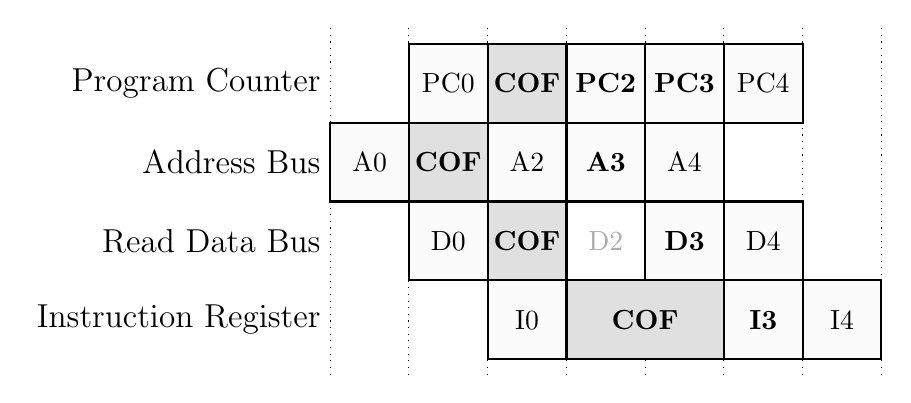
\begin{tikzpicture}

        %Lines
        \draw [dotted] (0,0.3) -- (0,4.7);
        \draw [dotted] (1,0.3) -- (1,4.7);
        \draw [dotted] (2,0.3) -- (2,4.7);
        \draw [dotted] (3,0.3) -- (3,4.7);
        \draw [dotted] (4,0.3) -- (4,4.7);
        \draw [dotted] (5,0.3) -- (5,4.7);
        \draw [dotted] (6,0.3) -- (6,4.7);
        \draw [dotted] (7,0.3) -- (7,4.7);

        %Program counter
        \node  [left] at (0,4) {\large{Program Counter}};
        \draw [thick, fill=gray!3] (1,4.5) rectangle (2,3.5);
        \node at (1.5,4)  {PC0};
        \draw [thick, fill=gray!24] (2,4.5) rectangle (3,3.5);
        \node at (2.5,4)  {\textbf{COF}};
        \draw [thick, fill=gray!3] (3,4.5) rectangle (4,3.5);
        \node at (3.5,4)  {\textbf{PC2}};
        \draw [thick, fill=gray!3] (4,4.5) rectangle (5,3.5);
        \node at (4.5,4)  {\textbf{PC3}};
        \draw [thick, fill=gray!3] (5,4.5) rectangle (6,3.5);
        \node at (5.5,4)  {PC4};
        
        %Address bus
        \node [left] at (0,3) {\large{Address Bus}};
        \draw [thick, fill=gray!3] (0,3.5) rectangle (1,2.5);
        \node at (0.5,3)  {A0};
        \draw [thick, fill=gray!24] (1,3.5) rectangle (2,2.5);
        \node at (1.5,3)  {\textbf{COF}};
        \draw [thick, fill=gray!3] (2,3.5) rectangle (3,2.5);
        \node at (2.5,3)  {A2};
        \draw [thick, fill=gray!3] (3,3.5) rectangle (4,2.5);
        \node at (3.5,3)  {\textbf{A3}};
        \draw [thick, fill=gray!3] (4,3.5) rectangle (5,2.5);
        \node at (4.5,3)  {A4};

        %Read data bus
        \node [left] at (0,2) {\large{Read Data Bus}};
        \draw [thick, fill=gray!3] (1,2.5) rectangle (2,1.5);
        \node at (1.5,2)  {D0};
        \draw [thick, fill=gray!24] (2,2.5) rectangle (3,1.5);
        \node at (2.5,2)  {\textbf{COF}};
        \draw [thick] (3,2.5) rectangle (4,1.5);
        \node [text=gray!64] at (3.5,2)  {D2};
        \draw [thick, fill=gray!3] (4,2.5) rectangle (5,1.5);
        \node at (4.5,2)  {\textbf{D3}};
        \draw [thick, fill=gray!3] (5,2.5) rectangle (6,1.5);
        \node at (5.5,2)  {D4};

        %Instruction register
        \node [left] at (0,1) {\large{Instruction Register}};
        \draw [thick, fill=gray!3] (2,1.5) rectangle (3,0.5);
        \node at (2.5,1)  {I0};
        \draw [thick, fill=gray!24] (3,1.5) rectangle (5,0.5);
        \node at (4,1)  {\textbf{COF}};
        \draw [thick, fill=gray!3] (5,1.5) rectangle (6,0.5);
        \node at (5.5,1)  {\textbf{I3}};
        \draw [thick, fill=gray!3] (6,1.5) rectangle (7,0.5);
        \node at (6.5,1)  {I4};

      \end{tikzpicture}
    }
  }
  \caption{Execution of a Change of Flow Instruction}
  \label{architecture:excyc:cof:fig}
  \end{center}
\end{figure}


\subsubsection{Exceptions and Interrupts}
\label{architecture:excyc:excpt}

%Exceptions
TBD

\begin{figure}[!h]
  \begin{center}
  \makebox[\textwidth][c]{
  \scalebox{1} {
      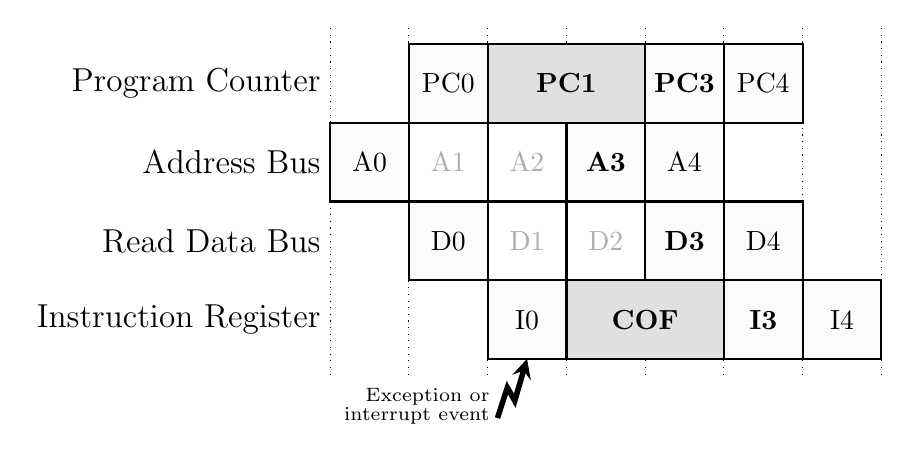
\begin{tikzpicture}

        %Lines
        \draw [dotted] (0,0.3) -- (0,4.7);
        \draw [dotted] (1,0.3) -- (1,4.7);
        \draw [dotted] (2,0.3) -- (2,4.7);
        \draw [dotted] (3,0.3) -- (3,4.7);
        \draw [dotted] (4,0.3) -- (4,4.7);
        \draw [dotted] (5,0.3) -- (5,4.7);
        \draw [dotted] (6,0.3) -- (6,4.7);
        \draw [dotted] (7,0.3) -- (7,4.7);

        %Program counter
        \node  [left] at (0,4) {\large{Program Counter}};
        \draw [thick, fill=gray!3] (1,4.5) rectangle (2,3.5);
        \node at (1.5,4)  {PC0};
        \draw [thick, fill=gray!24] (2,4.5) rectangle (4,3.5);
        \node at (3,4)  {\textbf{PC1}};
        %\draw [thick] (3,4.5) rectangle (4,3.5);
        %\node [text=gray!64] at (3.5,4)  {PC1};
        \draw [thick, fill=gray!3] (4,4.5) rectangle (5,3.5);
        \node at (4.5,4)  {\textbf{PC3}};
        \draw [thick, fill=gray!3] (5,4.5) rectangle (6,3.5);
        \node at (5.5,4)  {PC4};
        
        %Address bus
        \node [left] at (0,3) {\large{Address Bus}};
        \draw [thick, fill=gray!3] (0,3.5) rectangle (1,2.5);
        \node at (0.5,3)  {A0};1
        \draw [thick] (1,3.5) rectangle (2,2.5);
        \node [text=gray!64] at (1.5,3)  {A1};
        \draw [thick] (2,3.5) rectangle (3,2.5);
        \node [text=gray!64]  at (2.5,3)  {A2};
        \draw [thick, fill=gray!3] (3,3.5) rectangle (4,2.5);
        \node at (3.5,3)  {\textbf{A3}};
        \draw [thick, fill=gray!3] (4,3.5) rectangle (5,2.5);
        \node at (4.5,3)  {A4};

        %Read data bus
        \node [left] at (0,2) {\large{Read Data Bus}};
        \draw [thick, fill=gray!3] (1,2.5) rectangle (2,1.5);
        \node at (1.5,2)  {D0};
        \draw [thick] (2,2.5) rectangle (3,1.5);
        \node [text=gray!64] at (2.5,2)  {D1};
        \draw [thick] (3,2.5) rectangle (4,1.5);
        \node [text=gray!64] at (3.5,2)  {D2};
        \draw [thick, fill=gray!3] (4,2.5) rectangle (5,1.5);
        \node at (4.5,2)  {\textbf{D3}};
        \draw [thick, fill=gray!3] (5,2.5) rectangle (6,1.5);
        \node at (5.5,2)  {D4};

        %Instruction register
        \node [left] at (0,1) {\large{Instruction Register}};
        \draw [thick, fill=gray!3] (2,1.5) rectangle (3,0.5);
        \node at (2.5,1)  {I0};
        \draw [thick, fill=gray!24] (3,1.5) rectangle (5,0.5);
        \node at (4,1)  {\textbf{COF}};
        \draw [thick, fill=gray!3] (5,1.5) rectangle (6,0.5);
        \node at (5.5,1)  {\textbf{I3}};
        \draw [thick, fill=gray!3] (6,1.5) rectangle (7,0.5);
        \node at (6.5,1)  {I4};

        %Exception
        \draw [line width=2pt,-stealth] (2.125,-0.25) -- (2.25,0.135) -- (2.34375,-0.03125) -- (2.5,0.5);
        \node [align=right] at (1.1,-0.1) {\scriptsize{Exception or} \\[-5pt] \scriptsize{interrupt event}};

        
      \end{tikzpicture}
    }
  }
  \caption{Program flow interruted by an exception - TBD}
  \label{architecture:excyc:excpt:fig}
  \end{center}
\end{figure}


\subsection{Design Components}
\label{architecture:comp}

The N1 architecture is divided in 11 subblocks as shown in \figref{architecture:comp:fig}.

\begin{figure}[!h]
  \begin{center}
  \makebox[\textwidth][c]{
  \scalebox{1} {
      
\begin{tikzpicture}

        \node [left] at (0,0) {\large{TBD}};

      \end{tikzpicture}
    }
  }
  \caption{Block Diagram}
  \label{architecture:comp:fig}
  \end{center}
\end{figure}


\subsubsection{Flow Control Block (\texttt{fc})}
\label{architecture:fc}

The flow control block is implemented in the Verilog module \texttt{N1\_fc} (N1\_fc.v).
It manages the  \hyperref[architecture:excyc]{instruction cycles} of the N1 core.
It handles the control and resonse signals of the  \hyperref[integration:if:pbus]{program bus's} \gls{wb} interface and
it communicates with the other N1 componenents by sending requests and receiving status information.
No actual data passes through the \texttt{N1\_fc} module.
The interfaces to the N1 compunents, which are under the control of the flow control block, are explained in the following sections.

\paragraph{Control and Status Interface to the \hyperref[architecture:comp:ir]{Instruction Register}} \mbox{} \\
\label{architecture:fc:irif}

The flow control block is able to request has the following request signals to the instruction register: 
\begin{description}[style=nextline]

\item[\texttt{fc2ir\_capture}]
Capture the \hyperref[integration:if:pbus]{program bus's} read data (\texttt{pbus\_dat\_i}) in the
instruction register at the next clock edge.

\item[\texttt{fc2ir\_stash}]
Capture the \hyperref[integration:if:pbus]{program bus's} read data (\texttt{pbus\_dat\_i}) in the
stash register at the next clock edge.

\item[\texttt{fc2ir\_expend}]
The read data input of the \hyperref[integration:if:pbus]{Program Bus (\texttt{pbus\_dat\_i})}

\item[\texttt{fc2ir\_expend}]
Copy the stash regiesr's content into the instruction register at the next clock cycle.

\end{description}

The following status signala are coming from the instruction register:
%\begin{description}[style=nextline]
%\end{description}


\subsubsection{Instruction Register (\texttt{ir})}
\label{architecture:comp:ir}







%\subsubsection{Incoming Information}
%\label{architecture:ir:in}
%
%\subsubsection{Outgoing Information}
%\label{architecture:ir:out}

\subsubsection{Arithmetic Logic Unit (\texttt{alu})}
\label{architecture:comp:alu}

TBD

%\subsubsection{Incoming Information}
%\label{architecture:alu:in}

%\subsubsection{Outgoing Information}
%\label{architecture:alu:out}

\subsubsection{DSP Block (\texttt{dsp})}
\label{architecture:comp:dsp}

TBD

%\subsubsection{Incoming Information}
%\label{architecture:alu:in}

%\subsubsection{Outgoing Information}
%\label{architecture:alu:out}

\subsubsection{Exception Handler (\texttt{excpt})}
\label{architecture:comp:excpt}

TBD

%\subsubsection{Incoming Information}
%\label{architecture:alu:in}

%\subsubsection{Outgoing Information}
%\label{architecture:alu:out}

\subsubsection{Upper Stack (\texttt{us})}
\label{architecture:comp:us}

TBD

%\subsubsection{Incoming Information}
%\label{architecture:us:in}

%\subsubsection{Outgoing Information}
%\label{architecture:us:out}

\subsubsection{Intermediate Parameter Stack (\texttt{ips})}
\label{architecture:comp:ips}

TBD

%\subsubsection{Incoming Information}
%\label{architecture:ips:in}

%\subsubsection{Outgoing Information}
%\label{architecture:ips:out}

\subsubsection{Intermediate Return Stack (\texttt{irs})}
\label{architecture:comp:irs}

TBD

%\subsubsection{Incoming Information}
%\label{architecture:irs:in}

%\subsubsection{Outgoing Information}
%\label{architecture:irs:out}

\subsubsection{Lower Stack (\texttt{ls})}
\label{architecture:comp:ls}

TBD

%\subsubsection{Incoming Information}
%\label{architecture:ls:in}

%\subsubsection{Outgoing Information}
%\label{architecture:ls:out}



%--------------------
% Verification 
%--------------------
\include{N1_verification}

%--------------------
% Tool summary
%--------------------
\include{N1_tools}

%--------------------
% Glossary
%--------------------
%\clearpage
\setglossarystyle{altlist}
\printglossaries

%--------------------
% Bibliography
%--------------------
\clearpage
%\phantomsection
%\addcontentsline{toc}{section}{References}
\section{References}
\bibliographystyle{plain}
\renewcommand{\section}[2]{}%
\bibliography{N1.bib}

\end{document}
